\chapter{Signal and control regions}

\section{Event selection}

\subsection{Trigger selection}
\label{sec:HLTsel}

The events are required to have fired the High-Level Trigger (HLT) paths described in section~\ref{sec:trigpaths}. Unlike in the Run 1 analysis, the trigger requirement in the Run 2 analysis does not depend on the selected final state. Instead, it is always the OR of all ten HLT paths, since associated production modes that can have additional leptons will be targeted. This improves the trigger efficiency further.

\subsection{Vertex selection}
\label{sec:vertexsel}

The events are required to have at least one good primary
vertex (PV) fullfilling all three of the following criteria: a high number of degrees
of freedom ($N_{PV}>4$), collisions restricted along the $z$-axis
($z_{PV}<24$ cm), and a small radius of the PV ($r_{PV}<2$ cm).


\subsection{$ZZ$ candidate selection}
\label{sec:zzcandsel}

The four-lepton candidates are built from what we call "selected" leptons, which  
are the tight leptons (defined in Sections~\ref{sec:eleID} and~\ref{sec:muonReco}) that pass the ${\rm SIP_{3D}} < 4$ vertex constraint
and the isolation cuts (defined in Sections~\ref{sec:eleiso} and~\ref{sec:muoniso}), 
where FSR photons are subtracted as described in Section~\ref{sec:FSRphotons}.
A lepton cross-cleaning is applied 
by discarding electrons that are within $\Delta R < 0.05$ of selected muons. 


The construction and selection of four-lepton candidates proceeds 
according to the following sequence:
\begin{enumerate}
\item {\bf $Z$ candidates} are defined as pairs of selected leptons
 of opposite charge and matching flavor (e.g. $e^+ e^-$ or $\mu^+\mu^-$)
 that satisfy $12 < m_{\ell\ell(\gamma)} < 120~\GeV$, where the $Z$ candidate mass
 includes the selected FSR photons if any.
\item {\bf $ZZ$ candidates} are defined as pairs of non-overlapping $Z$ candidates.
 The $Z$ candidate with reconstructed mass $m_{\ell\ell}$ closest to the nominal $Z$ boson
 mass is denoted as $\Z_1$, and the second one is denoted as $Z_2$. The dimuon distributions for $Z_1$ and $Z_2$ are shown in Figure~\ref{fig:dimuonz1} and Figure~\ref{fig:dimuonz2}, respectively. The dielectron distributions are qualitatively the same.

\begin{figure}[tbh]
\centering
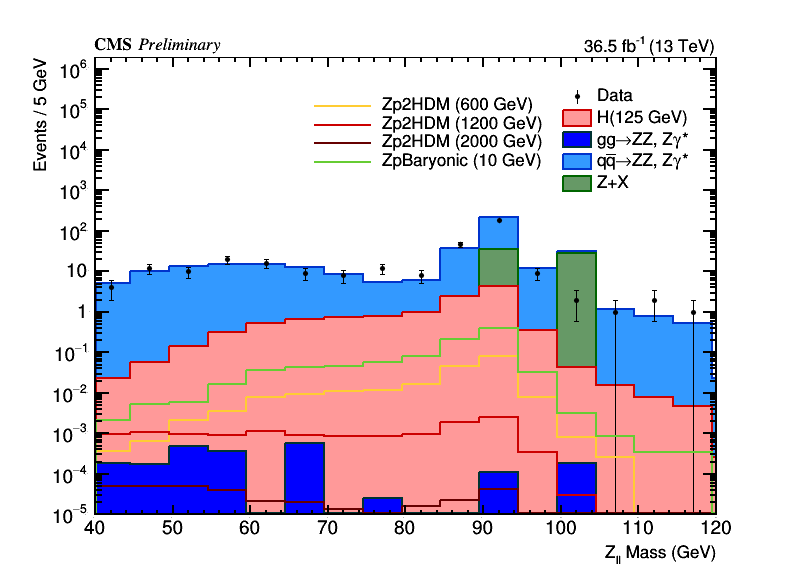
\includegraphics[width=5.5in]{figures/hist_hMZ1_8.png}
    \caption{Dimuon invariant mass distributions for ${\rm Z_1}$.}
    \label{fig:dimuonz1}
\end{figure}

\begin{figure}[tbh]
\centering
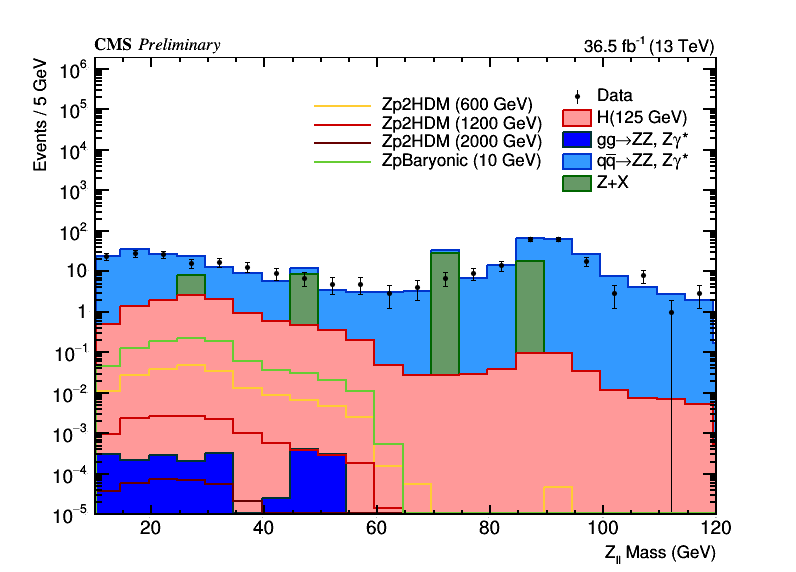
\includegraphics[width=5.5in]{figures/hist_hMZ2_8.png}
    \caption{Dimuon invariant mass distributions for ${\rm Z_2}$.}
    \label{fig:dimuonz2}
\end{figure}

$ZZ$ candidates are required to satisfy the following list of requirements:
  \begin{itemize} 
  \item {\bf Ghost removal }: $\Delta R(\eta,\phi) > 0.02$ between each of the four leptons
  \item {\bf Lepton $p_T$}: two of the four selected leptons should pass 
     $p_{T,i} > 20~\GeV$ and $p_{T,j} > 10~\GeV$
  \item {\bf QCD suppression}: all four oppositely-signed pairs that can
     be built with the four leptons (regardless of lepton flavor)
     must satisfy $m_{\ell\ell} > 4~\GeV$.
     Here, selected FSR photons are not used in computing $m_{\ell\ell}$, 
     since a QCD-induced low-mass dilepton (e.g. $J/\Psi$) 
     may have photons nearby (e.g. from $\pi_0$)
  \item {\bf $Z_1$ mass}: $m_{Z1} > 40~\GeV$
  \item {\bf `smart cut'}: defining $Z_a$ and $Z_b$ as 
     the mass-sorted alternative pairing $Z$ candidates 
     ($Z_a$ being the one closest to the nominal $Z$ boson mass),
     require NOT($|m_{ Za}-m_{ Z}| < |m_{ Z1}-m_{ Z}|$ AND $m_{ Zb}<12$).
     Selected FSR photons are included in $m_{ Z}$'s computations.
     This cut discards $4\mu$ and $4e$ candidates where the alternative pairing
     looks like an on-shell $Z$ + low-mass $\ell^+ \ell^-$. 
     In Run 1, such a situation was avoided by choosing the best $ZZ$ candidate
     before applying kinematic cuts to it, most precisely before the $m_{Z2} > 12~\GeV$ cut.
     The present smart cut allows to choose the best $ZZ$ candidate after all kinematic cuts.   
  \item {\bf Four-lepton invariant mass}: $\mllll > 70~\GeV$. The four-muon invariant mass distribution after all of the previous selection steps are applied is shown in Figure~\ref{fig:m4mulog}, with a close up view of the $Z$ and $H$ peaks shown in Figure~\ref{fig:m4mulin}. The four-lepton invariant mass distributions for the other decay channels are qualitatively the same
  \end{itemize}	
\item Events containing at least one selected $ZZ$ candidate form the SM signal region.
\end{enumerate}	

\begin{figure}[tbh]
\centering
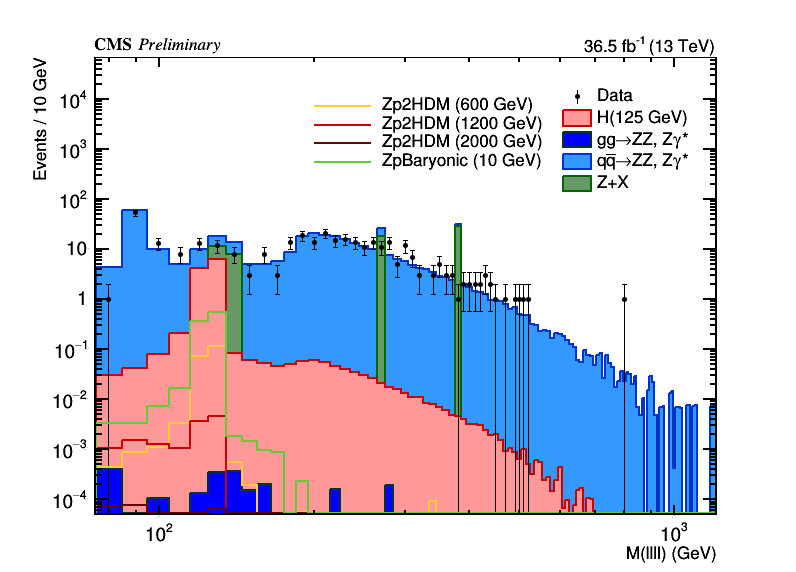
\includegraphics[width=5.5in]{figures/hist_hM4l_8_log.png}
    \caption{Four-muon invariant mass distribution in log scale.}
    \label{fig:m4mulog}
\end{figure}

\begin{figure}[tbh]
\centering
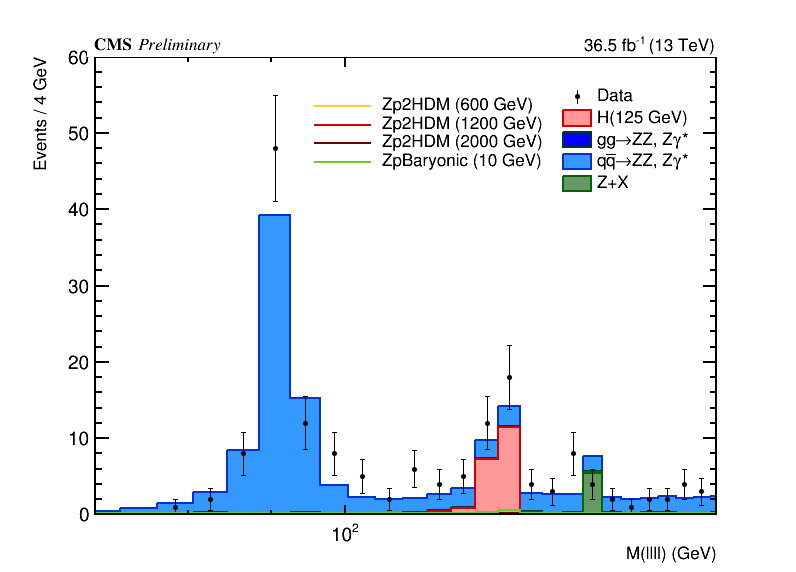
\includegraphics[width=5.5in]{figures/hist_hM4l_8_linear.png}
    \caption{Four-muon invariant mass distribution in linear scale.}
    \label{fig:m4mulin}
\end{figure}

\subsection{Choice of the best $ZZ$ candidate}
\label{sec:zzbestcand}

Unlike in the Run 1 analysis, the best $ZZ$ candidate in the Run 2 analysis is chosen after all kinematic cuts, a change that allows to test other selection strategies for this candidate choice. 
This is especially relevant for events with more than four selected leptons, such as $VH$ and $ttH$, with associated particles that can decay to additional leptons.

For the current analysis, if more than one $ZZ$ candidate survives the above selection,
we choose the one with the highest value of $\KD$, the MELA kinematic discriminant, except if
two candidates are composed of four leptons, in which case, the candidate with $Z_1$ closest in mass to nominal 
$Z$ boson mass is chosen.


\section{Signal region and blinding}

A one-step SR and optimization process is used in the current analysis, where a near-optimal SR is defined using all of the desired variables, instead of the two-step procedure used in previous anlayses. This simplification allows for the use of the same SR for all signal models, including the same variable validation and background model. The tradeoff is a small loss in sensitivity for models with tighter optimal cuts, but the benefit of simplicity outweighs the cost of this loss. In principle, each benchmark signal point can be optimized individually to gain a few percent in sensitivity, but this is left to a future study.

Two strategies are employed to define the signal region: cut-and-count based and multivariate analysis (MVA) based. Several key discriminating variables are studied as inputs to both SR definitions: the missing transverse energy, $\MET$ or MET; the four-lepton invariant mass, $m_{4l}$; the transverse mass of the Higgs and MET, $m_T(4l+\MET) \equiv m_T$; the difference in the transverse angle $\phi$ between the Higgs and MET, $|\Delta\phi(4l, \MET)| \equiv |\Delta\phi|$; as well as the lepton and jet multiplicities.

\subsection{Cut-and-count based signal region} \label{cutandcountopt}

The cut-and-count strategy is the simpler choice and is used as a baseline to measure the performance of the MVA. First, the following selection is applied to isolate events with a Higgs from events with additional prompt particles (e.g. VBF Higgs production):

\begin{itemize}
\item Tight-lepton multiplicity = 4
\item b-jet multiplicity $\leq$ 1
\item VBF jet multiplicity $\leq$ 1.
\end{itemize}

Next, the event selection is optimized by scanning over a range of cuts for the remaining variables and selecting the set of cuts that maximizes the sensitivity, measured directly by the cross section upper limit. The two variables with the greatest discriminating power between signal and background are $m_{4l}$ and $\MET$, so we maximize the sensitivity over these two variables. The best sensitivity occurs where the upper limit is minimumized, at approximately:

\begin{itemize}
\item $|m_{4l} - m_H| < 10$ $\GeV$
\item $\MET > 60$ $\GeV$
\end{itemize}

These cuts define the SR, which is applied to all of the signals, losing less than 10\% sensitivity for the models with a tighter optimal cut on $\MET$. Since the signal used to defined the SR has the softest $\MET$ spectrum of all the signals, this SR corresponds to the most modest or, meaning no signal will be cut too hard, while most of the background is still removed. 

%\begin{figure}[tbh]
%\centering
%\includegraphics[width=3in]{figures/}
%\caption{PLACEHOLDER The optimized cut-and-count based selection for ZpBaryonic, defining the signal region for all models.}
%\label{fig:2dscan}
%\end{figure}

Note that there is no additional blinding on the MET distribution above a certain threshold, as was the case previously in similar searches. This is due primarily to the need to understand events that contribute large amounts of fake MET. This is covered thoroughly, including the procedure for removing these events from data, in Section~\ref{sec:fakemet}. In order to validate the modeling in these SRs, they are split into control regions (CR) based on the MET being above or below 60 $\GeV$, referred to as the high and low MET regions. 


\subsection{MVA-based signal region} \label{mvaopt}

This search channel has the advantage of having backgrounds that are easily reduced by applying cuts on the discriminating variables. It was observed in the study of the 2015 data and MC samples that applying additional cuts did not improve the sensitivity since the background levels were already sufficiently low. Applying cuts on additional variables reduced the signal efficiency, which in turn reduced the sensitivity. This is also observed with 2016 MC samples, where applying the $|\Delta\phi(llll, \MET|$ does not improve the sensitivity. These observations motivate the use of MVA techniques, which can take all of the desired variables as inputs, but do not reduce the signal efficiency. Although it is simpler to cut on these discriminating variables using the cut-and-count method, there is potential for significant improvement in the sensitivity with an MVA approach.

The SR event selection is optimized for the MVA-based case by training a boosted decision tree (BDT) with the ROOT TMVA package with $m_{4l}$ and $\MET$ the input variables. Including additional input features does not significantly improve the performance of the MVA. Training is done over the weighted set of simulated backgrounds and an admixture of signal models to reduce bias toward a single signal model. The BDT response is shown in Figure~\ref{fig:bdt}, with the signal peaked toward 1 and the background peaked toward $-1$. 

\begin{figure}[tbh]
\centering
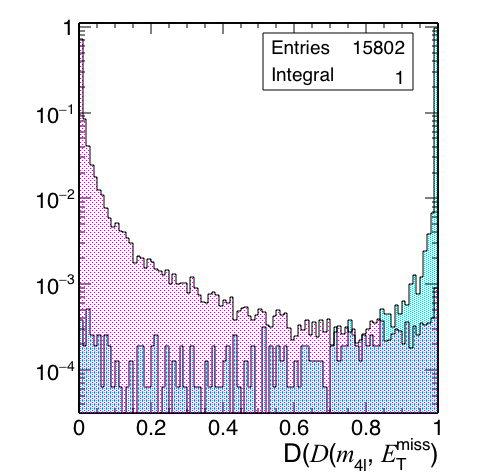
\includegraphics[width=5in]{figures/f_Dm4lmet_1D_log.png}
\caption{Boosted decision tree response trained on a weighted background sample and admixture of signal samples with input variables $m_{4l}$ and $\MET$. Simulated backgrounds are in pink and signals are in blue.}
\label{fig:bdt}
\end{figure}

\section{Background modeling}

\subsection{Irreducible backgrounds}
\label{sec:irrbkgd}

\subsubsection{$\qqZZ$ modeling}
\label{sec:redbkgd}

The $\qqZZ$ background is generated at NLO, while the fully differential cross section has been computed at 
NNLO~\cite{Grazzini2015407} but is not yet available in a partonic level event generator. Therefore, NNLO/NLO 
$k$-factors for the $\qqZZ$ background process are applied to the {\sc powheg} sample. The inclusive cross 
sections obtained using the same PDF and renormalization and factorization scales as the {\sc powheg} sample
at LO, NLO, and NNLO are shown in Table~\ref{tab:qqZZXS}. The NNLO/NLO $k$-factors are applied in the analysis
differentally as a function of $m(\cPZ\cPZ)$. 

Additional NLO electroweak corrections, which depend on the initial-state quark flavor and kinematics,
are also applied to the $\qqZZ$ background process in the region $m(\cPZ \cPZ)>2m(\cPZ)$. The differential QCD and electroweak $k$-factors can be seen in 
Figure~\ref{fig:qqZZKfactor}.

\begin{table}[h]
    \centering
    \begin{tabular}{|l|c|c|} 
\hline %----------------------------------------------------------------
QCD Order  & $\sigma_{2\ell2\ell^{\prime}} (\mathrm{fb})$  & $\sigma_{4\ell} (\mathrm{fb})$  \\
\hline %----------------------------------------------------------------
LO    & 218.5$^{+16\%}_{-15\%}$ & 98.4$^{+13\%}_{-13\%}$ \\
NLO   & 290.7$^{+5\%}_{-8\%}$   & 129.5$^{+4\%}_{-6\%}$ \\
NNLO  & 324.0$^{+2\%}_{-3\%}$   & 141.2$^{+2\%}_{-2\%}$ \\
\hline %----------------------------------------------------------------
    \end{tabular}
    \caption{Cross sections for $\qqZZ$ production at 13 \TeV}
    \label{tab:qqZZXS}
\end{table}

%=======
\begin{figure}[!htb]
\vspace*{0.3cm}
\begin{center}
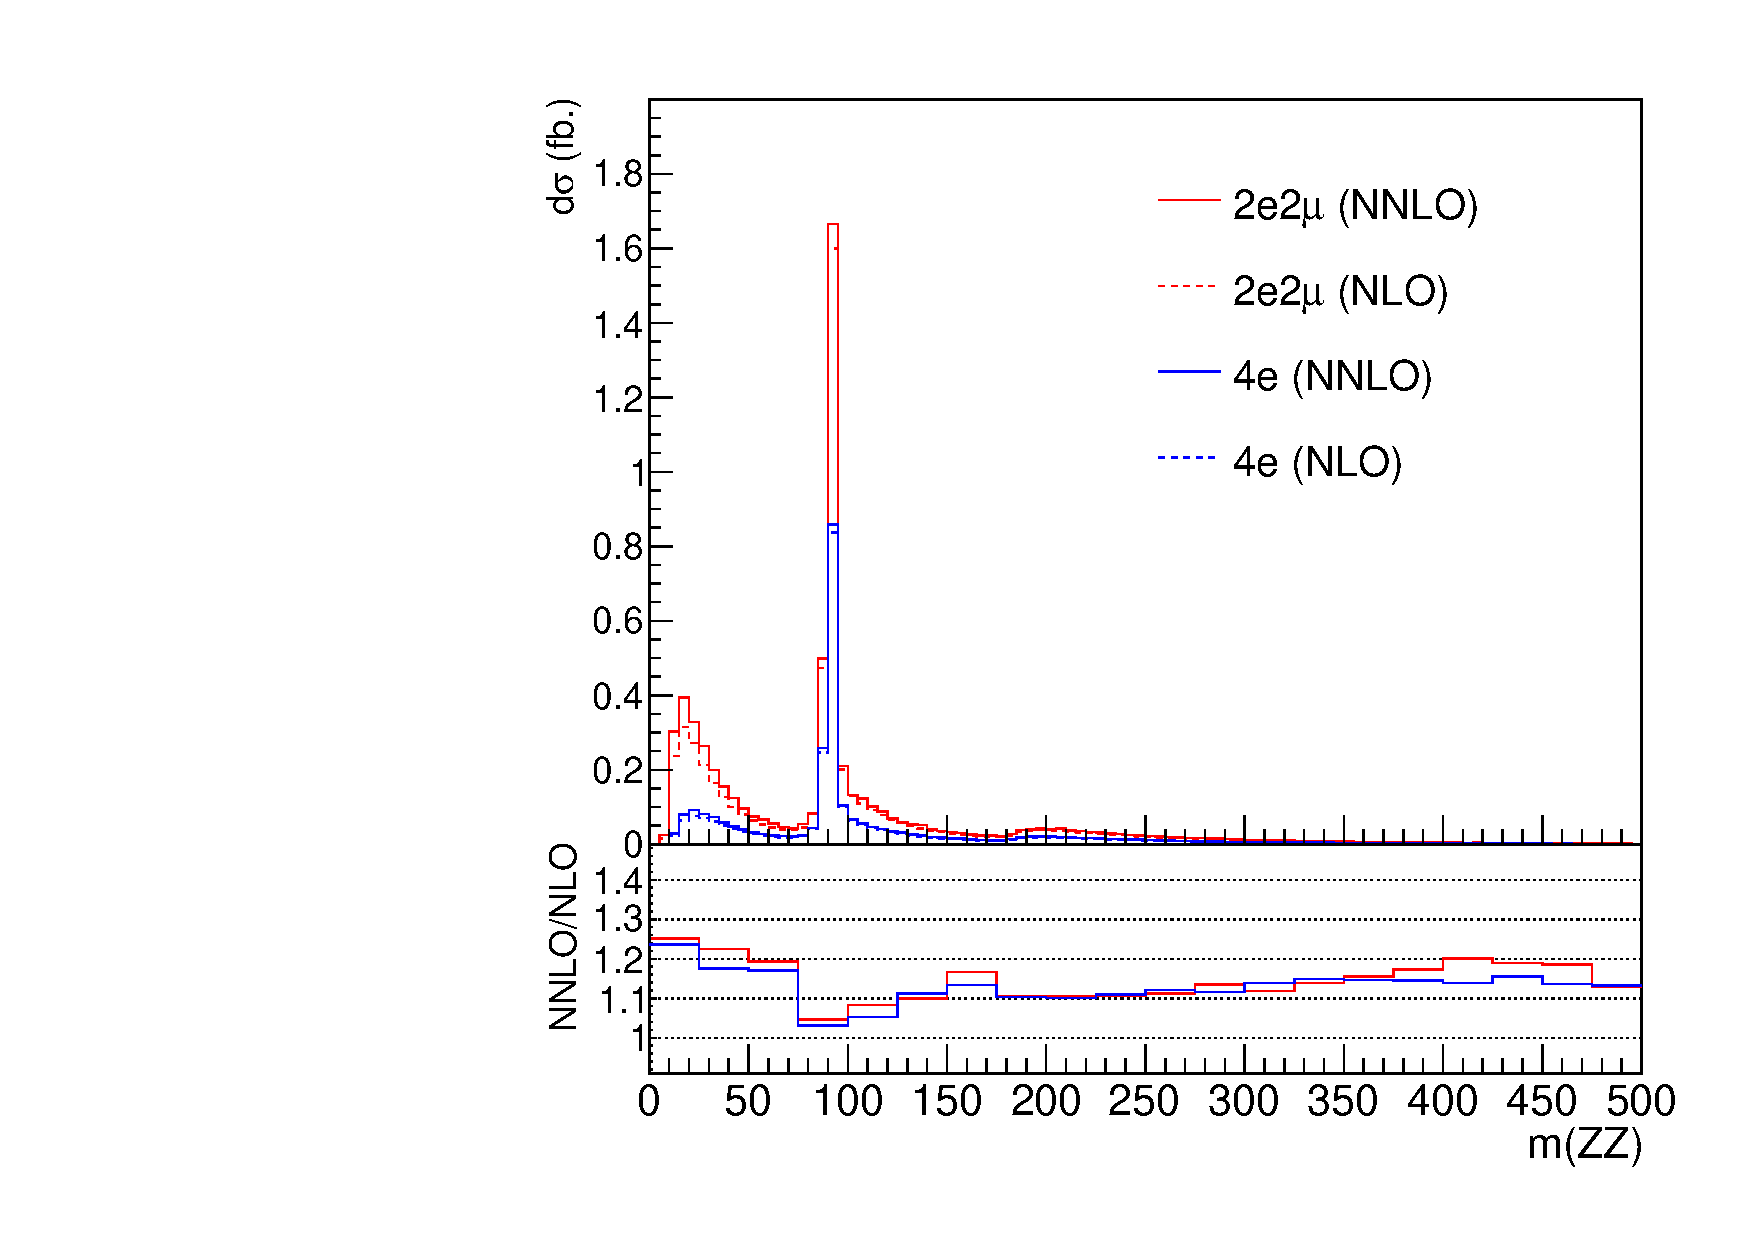
\includegraphics[width=0.48\textwidth]{Figures/IrrBkg/Kfactor_qqZZ_mZZ.pdf}
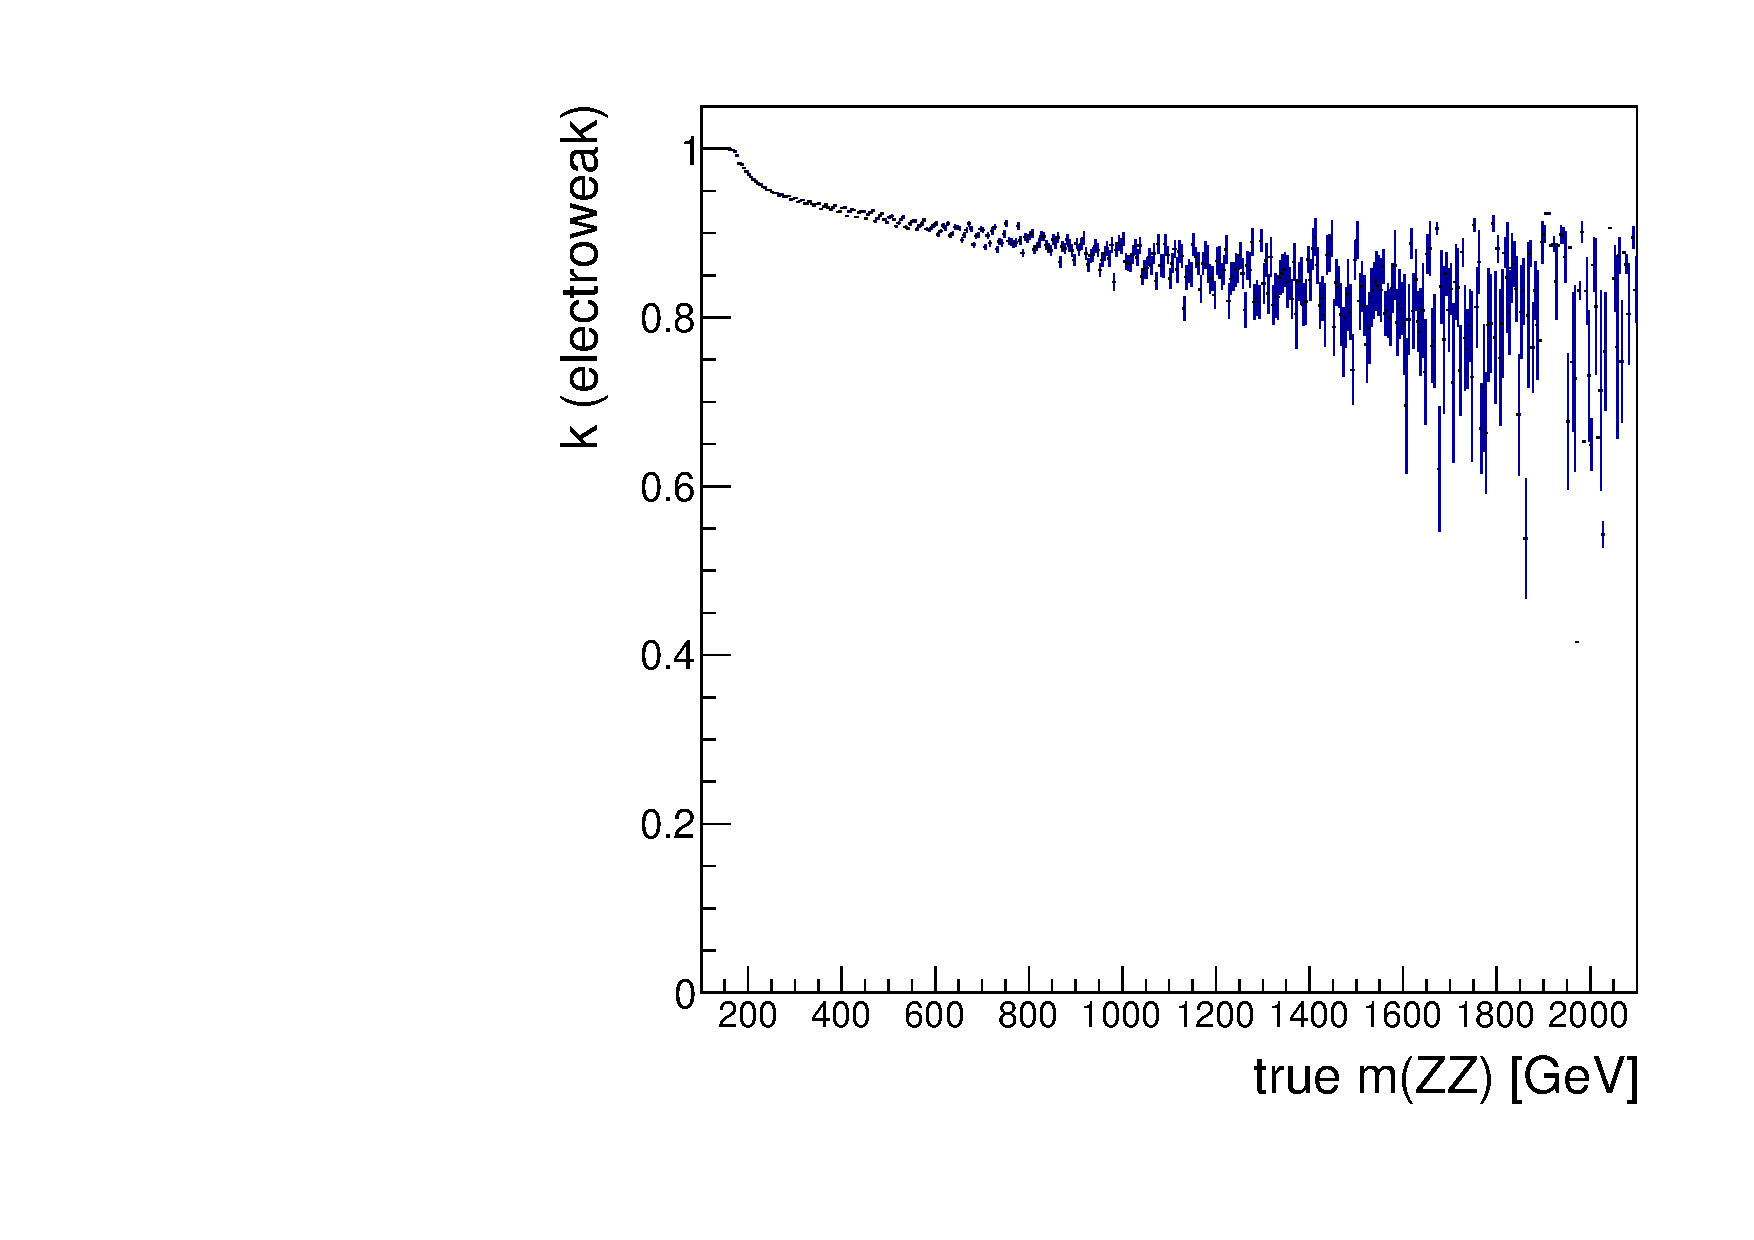
\includegraphics[width=0.48\textwidth]{Figures/IrrBkg/K_ewk_qqZZ.pdf} 
\caption{Left: NNLO/NLO QCD $k$-factor for the \qqZZ~ background as a function of $m(ZZ)$ for the $4\ell$ and $2\ell2\ell^{\prime}$ final states. Right: NLO/NLO electroweak $k$-factor for the \qqZZ~ background as a function of $m(ZZ)$.
\label{fig:qqZZKfactor}}
\end{center}
\end{figure}


\subsubsection{$\ggZZ$ modeling}

Event simulation for the $\ggZZ$ background is done at LO with the generator MCFM 7.0 \cite{MCFM,Campbell:2011bn,Campbell:2013una}.
Although no exact calculation exists beyond LO for the $\ggZZ$ background, 
it has been recently shown 
that the soft collinear approximation is able to describe the background cross section and the 
interference term at NNLO \cite{Bonvini:1304.3053}. Further calculations also show that the $k$-factors are very similar at NLO for the signal 
and background~\cite{Melnikov:2015laa} and at NNLO for the signal and interference terms~\cite{Li:2015jva}. Therefore, the same $k$-factor 
is used for the signal and background~\cite{Passarino:1312.2397v1}. The NNLO $k$-factor for the signal is obtained as a function of $\mllll$ 
using the \textsc{hnnlo}~v2 MC program~\cite{Catani:2007vq,Grazzini:2008tf,Grazzini:2013mca} by calculating the NNLO and LO 
$\Pg\Pg\to\PH\to2\ell2\ell^\prime$ cross sections at the small $\PH$ decay width of $4.07$ $\MeV$ and taking their ratios. The NNLO amd NLO $k$-factors and the cross sections from which they are derived are illustrated in Figure~\ref{fig:ggHZZXsecKfactor}, 
along with the NNLO, NLO and LO cross sections at the SM $\PH$ boson decay width~\cite{Heinemeyer:2013tqa}.
 
\begin{figure}[!htb]
\centering
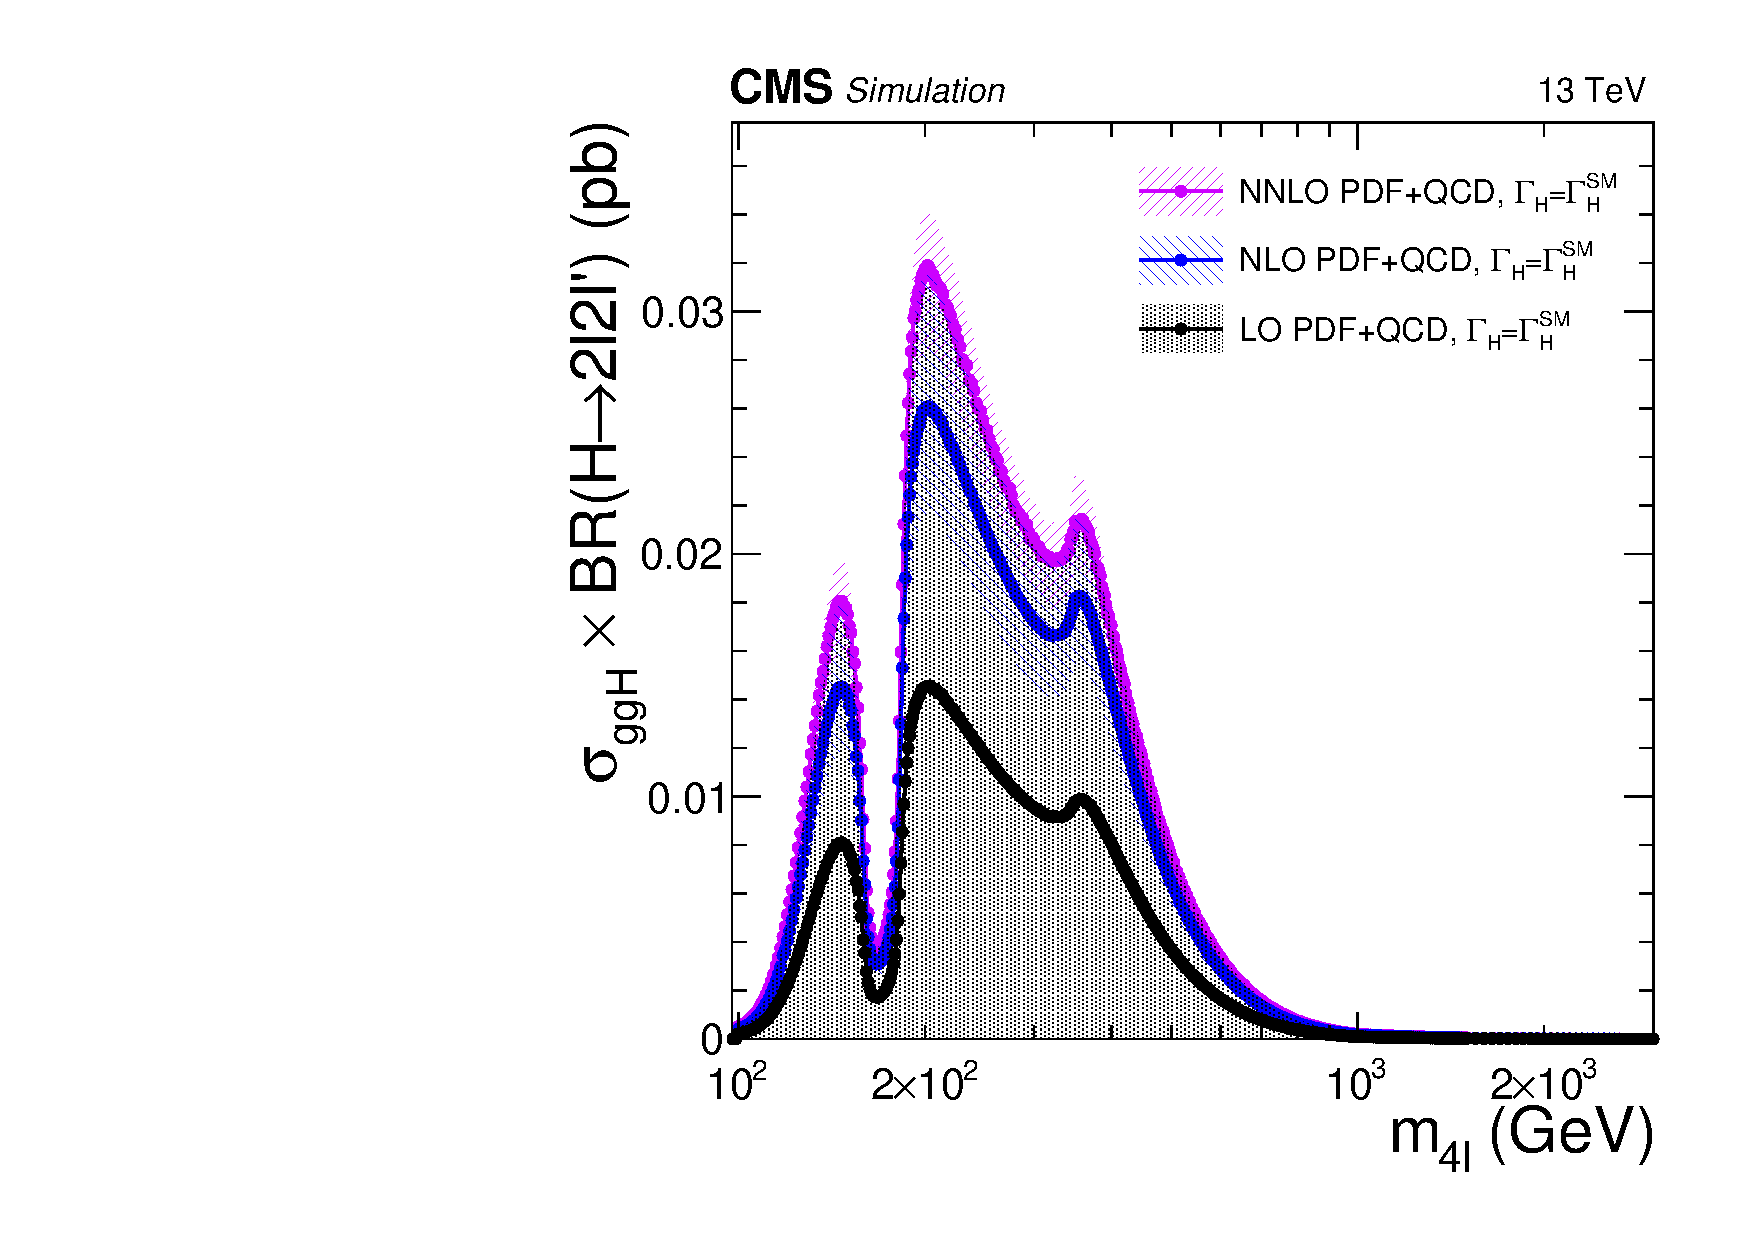
\includegraphics[width=0.48\linewidth]{Figures/IrrBkg/cCompare_hnnlo_ggHZZ2l2l_xsec.pdf}
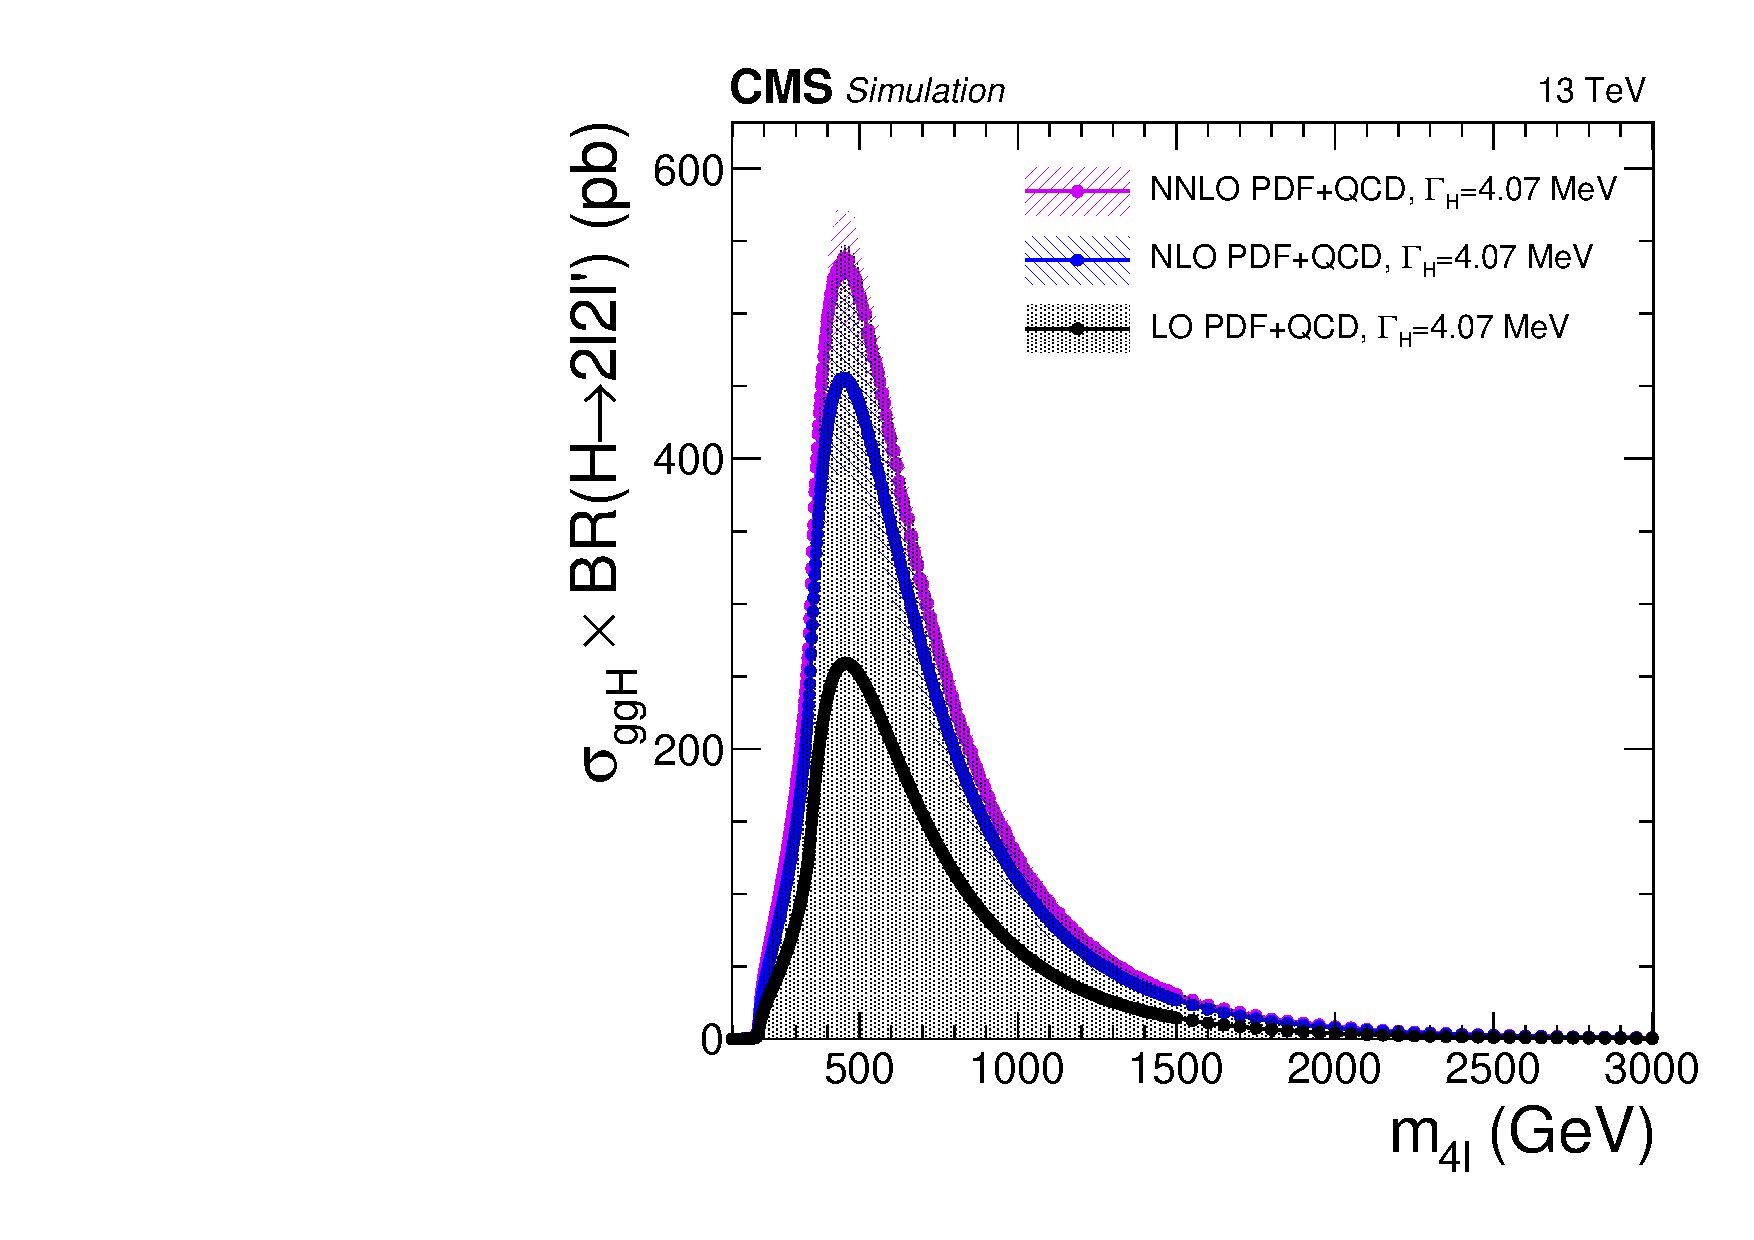
\includegraphics[width=0.48\linewidth]{Figures/IrrBkg/cCompare_hnnlo_ggHZZ2l2l_narrowwidth_xsec.pdf}\\
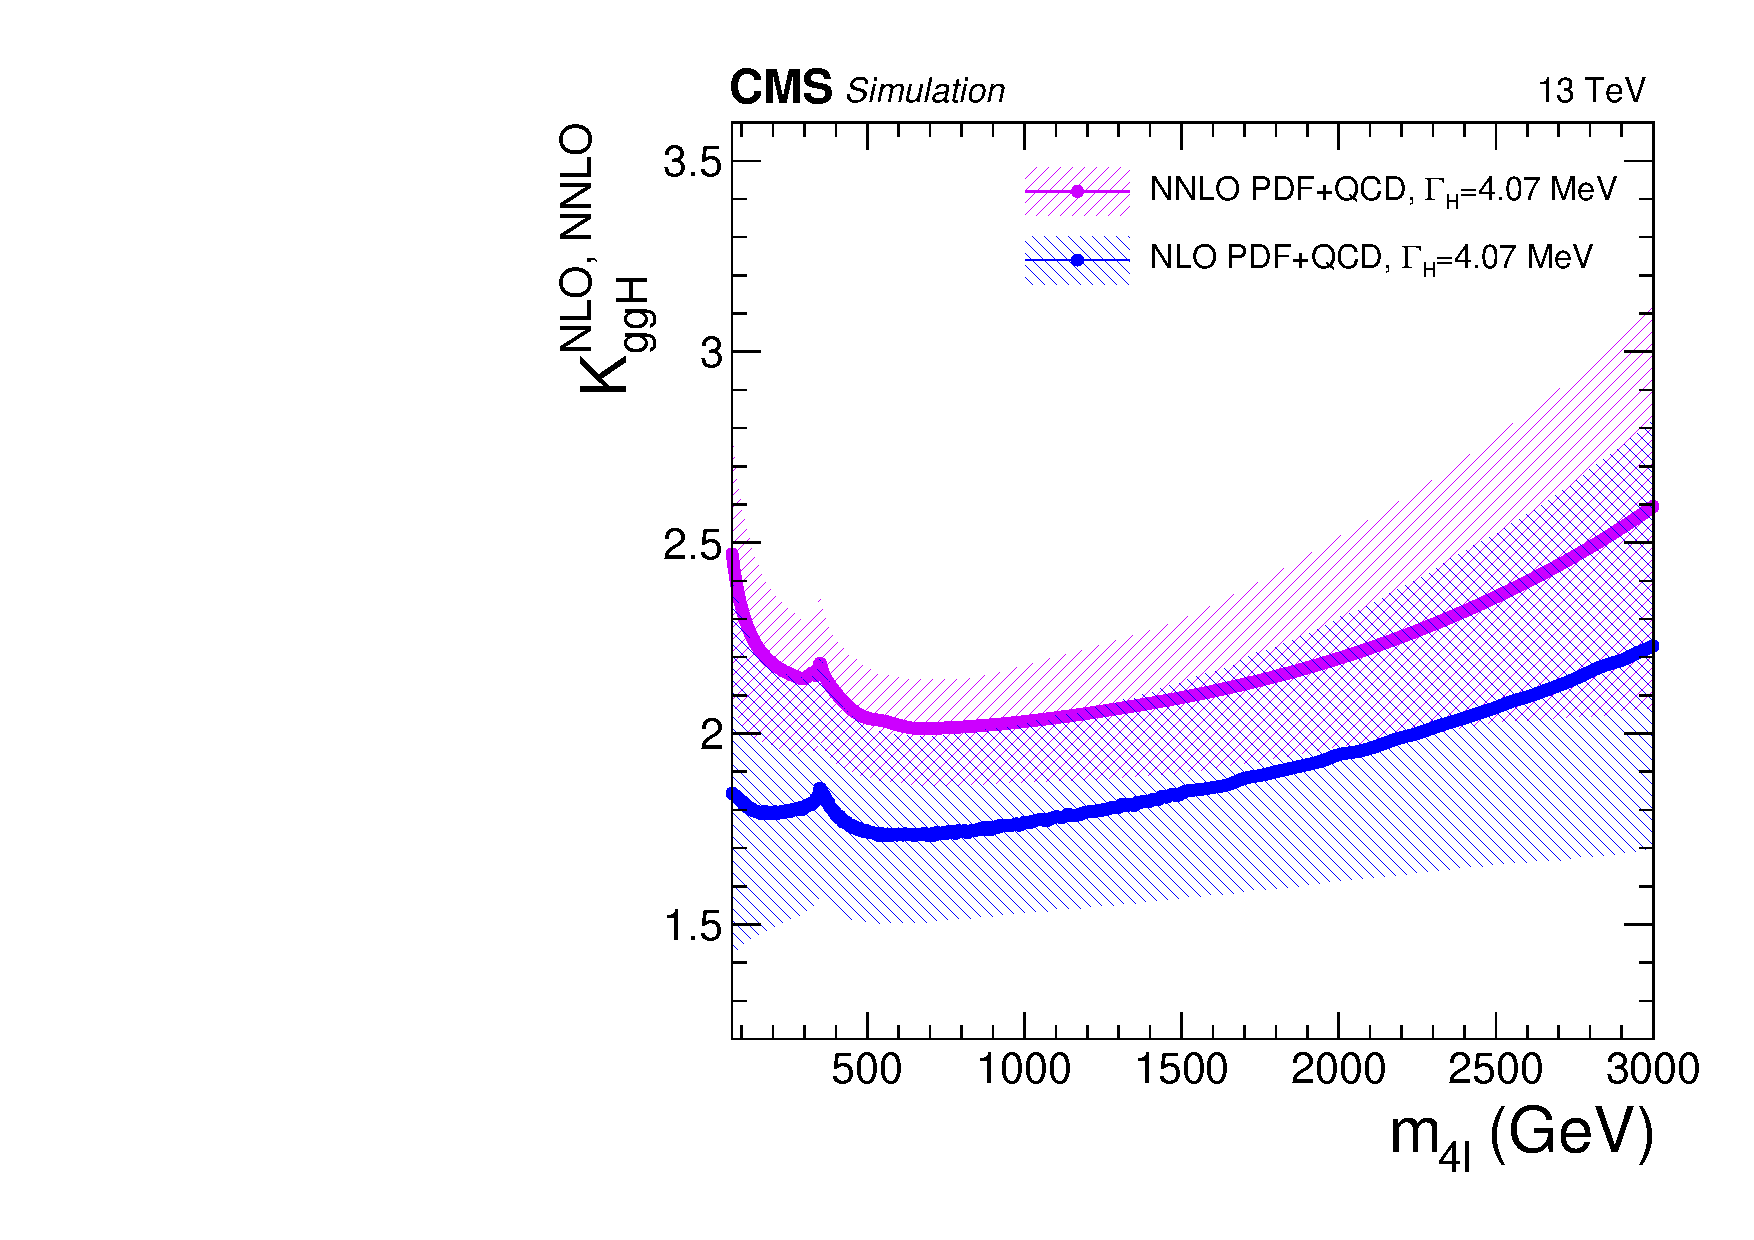
\includegraphics[width=0.48\linewidth]{Figures/IrrBkg/cCompare_hnnlo_ggHZZ2l2l_narrowwidth_kfactor.pdf}
\caption{$\Pg\Pg\to\PH\to2\ell2\ell^\prime$ cross sections at NNLO, NLO and LO at each $\PH$ pole mass using the SM $\PH$ decay width (top left) or at the fixed and small decay width of $4.07$ $\MeV$ (top right). The cross sections using the fixed value are used to obtain the $k$-factor for both the signal and the continuum background contributions as a function of $\mllll$ (bottom).
}
\label{fig:ggHZZXsecKfactor}
\end{figure}

%\begin{figure}[!htb]
%\centering
%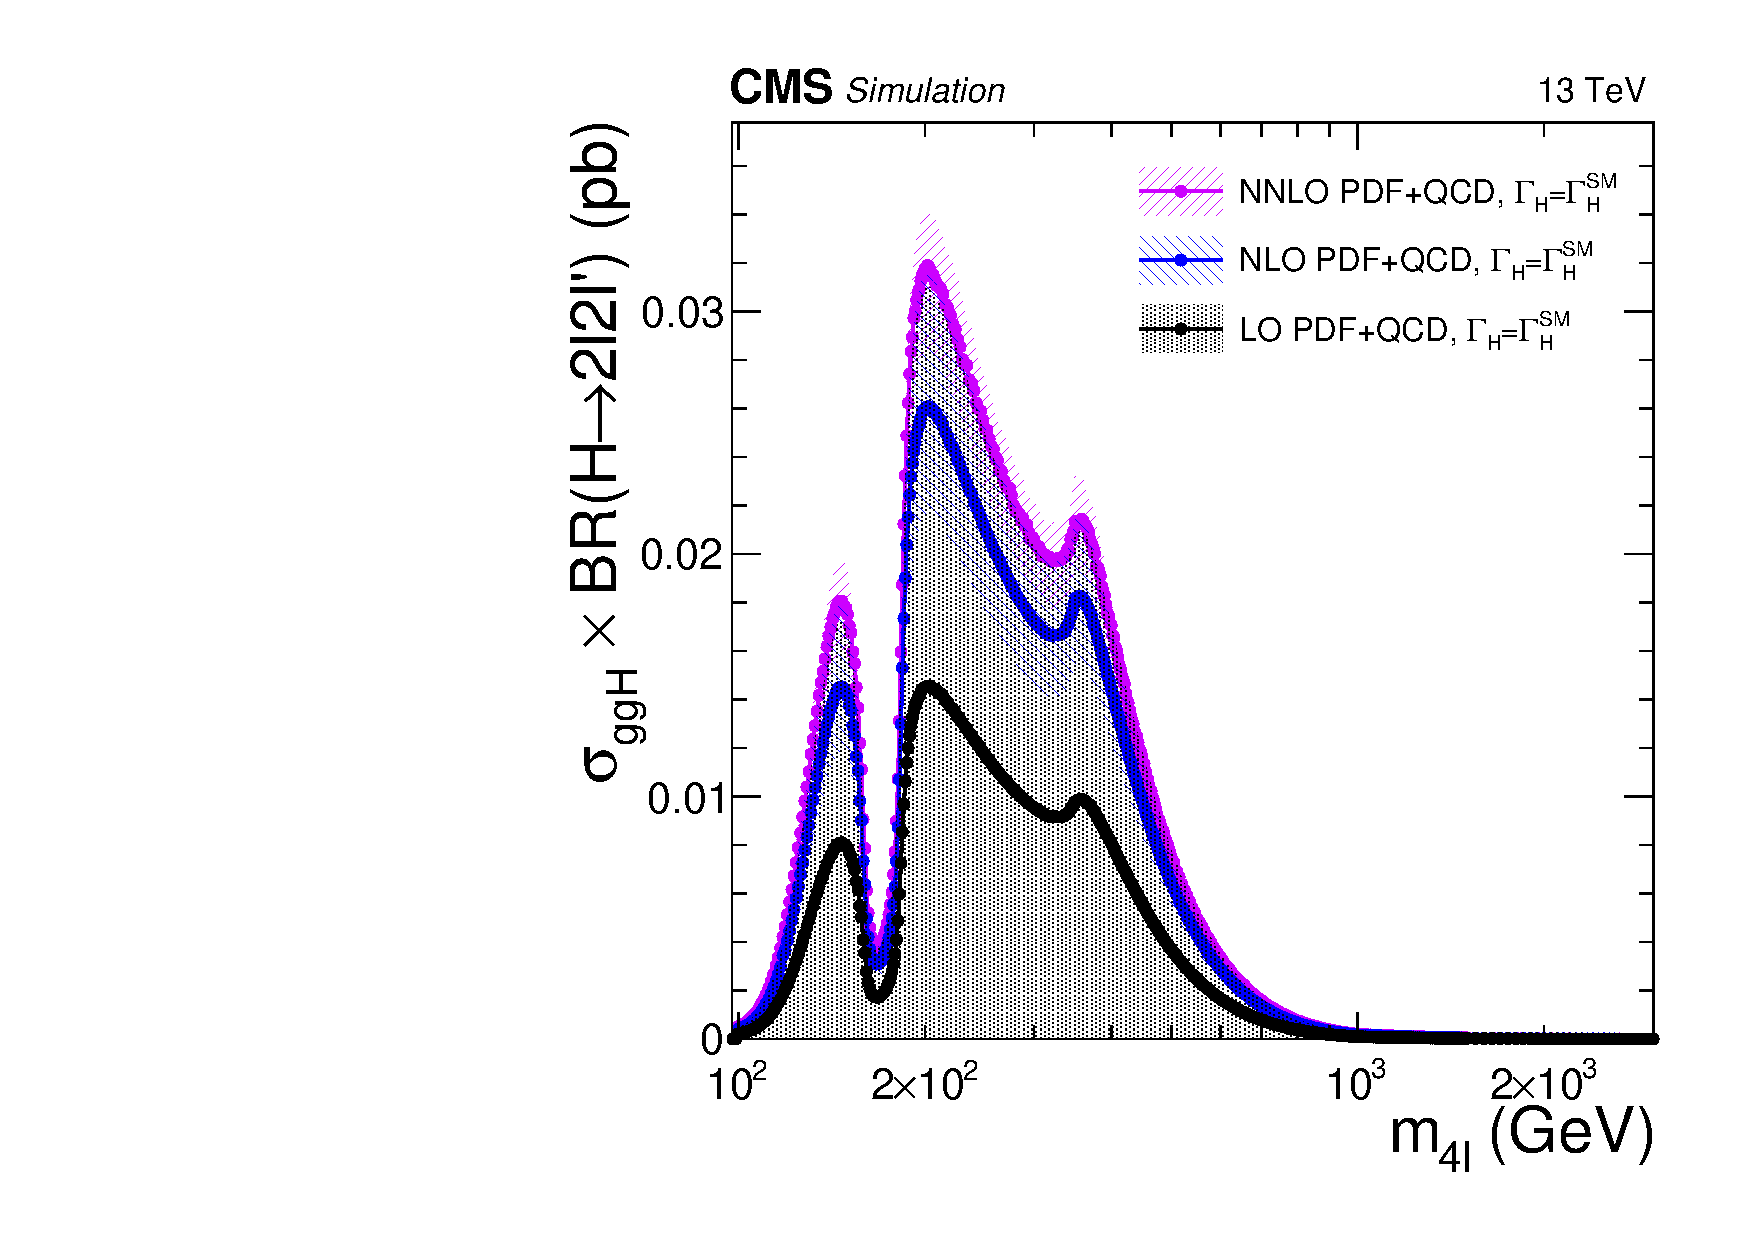
\includegraphics[width=0.48\linewidth]{Figures/IrrBkg/cCompare_hnnlo_ggHZZ2l2l_xsec.pdf}
%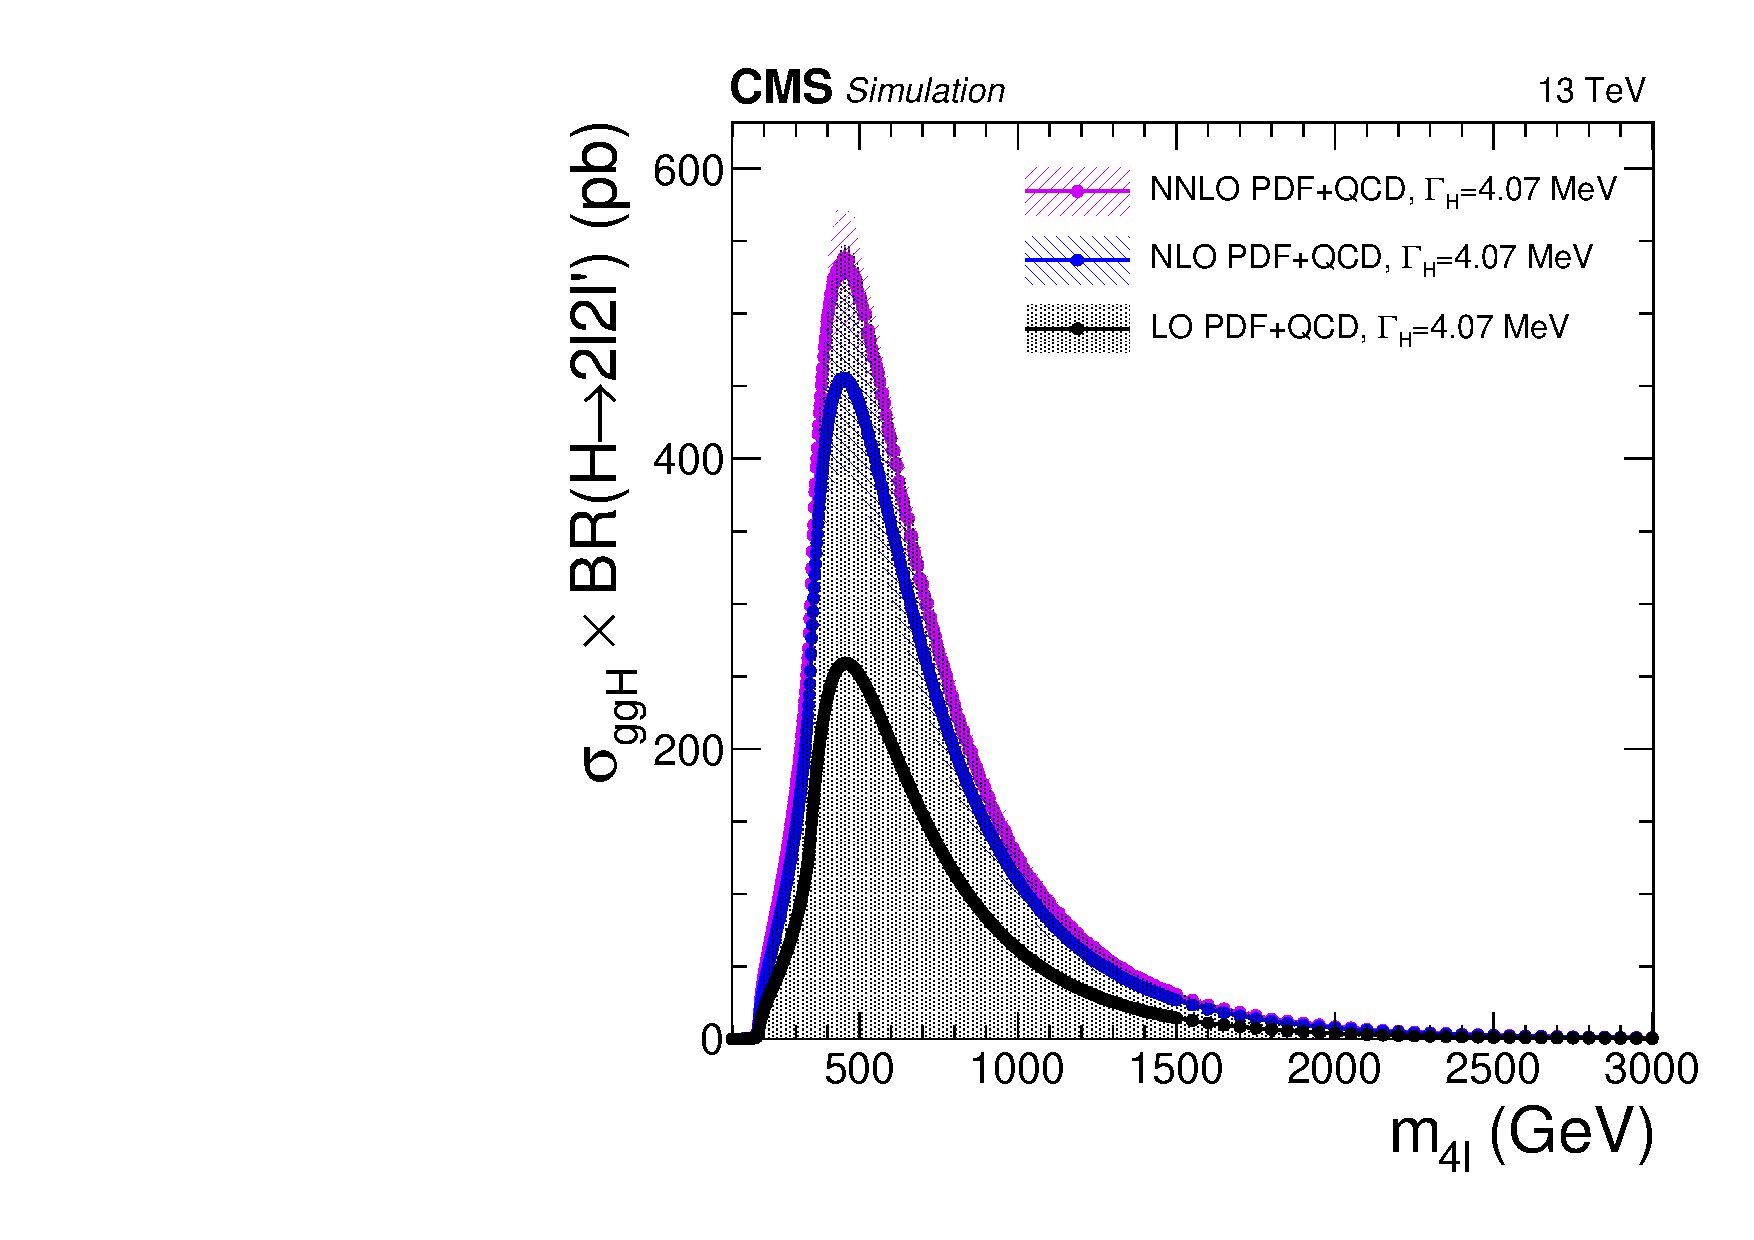
\includegraphics[width=0.48\linewidth]{Figures/IrrBkg/cCompare_hnnlo_ggHZZ2l2l_narrowwidth_xsec.pdf}\\
%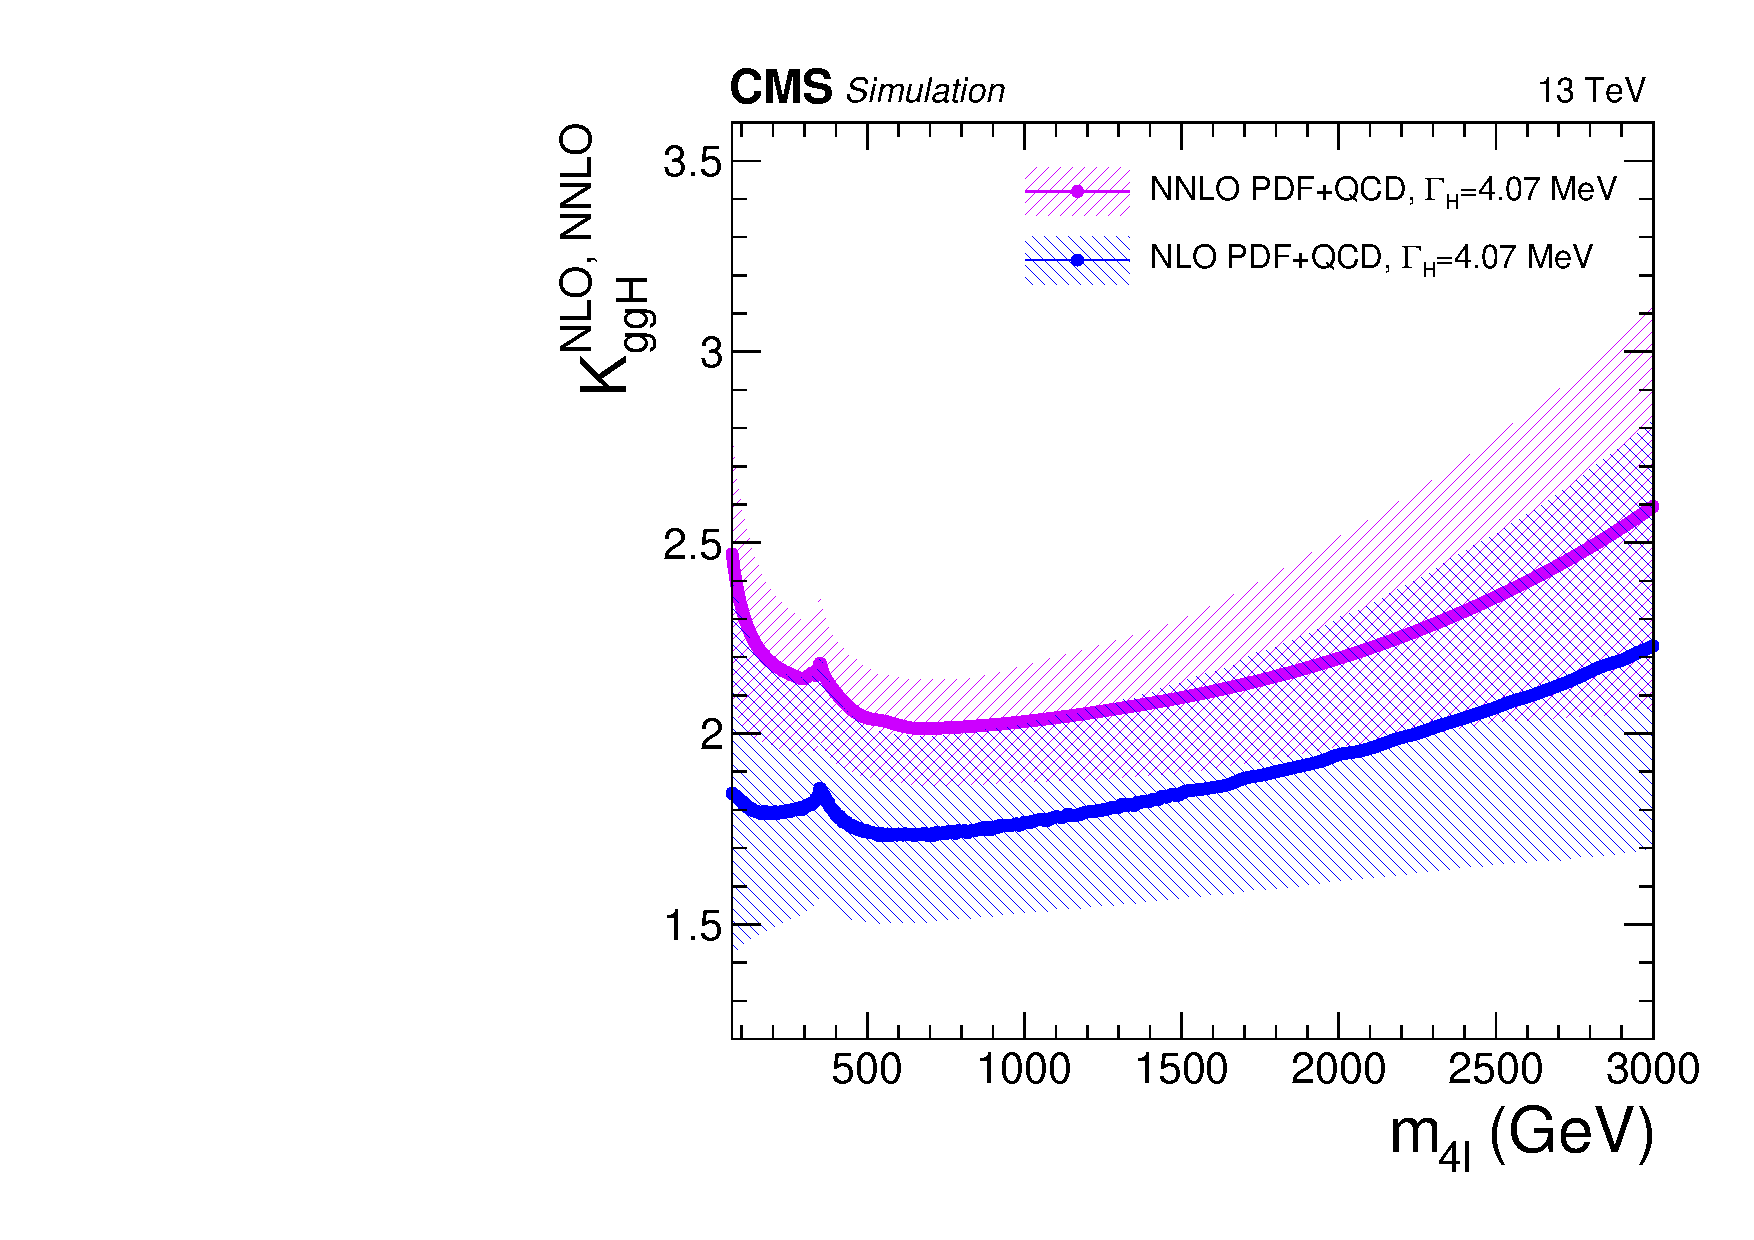
\includegraphics[width=0.48\linewidth]{Figures/IrrBkg/cCompare_hnnlo_ggHZZ2l2l_narrowwidth_kfactor.pdf}
%\caption{$\Pg\Pg\to\PH\to2\ell2\ell^\prime$ cross sections at NNLO, NLO and LO at each $\PH$ boson pole mass using the SM $\PH$ boson decay width  (top \cmsLeft) or at the fixed and small decay width of $4.07$~MeV (top \cmsRight). The cross sections using the fixed value are used to obtain the K factor for both the signal and the continuum background contributions as a function of $\mllll$ (bottom).
%}
%\label{fig:ggHZZXsecKfactor}
%\end{figure}

\subsection{Reducible background estimation}
\label{sec:zxIntr}
%\input{Background/zxIntr.tex}

The reducible background for the $H\to ZZ\to 4\ell $ analysis, hereafter called $Z+X$, originates from processes which contain one or more non-prompt lepton in the four-lepton final state. 
The main sources of non-prompt leptons are non-isolated electrons and muons coming from decays of heavy-flavor mesons, mis-reconstructed jets (usually originating from light-flavor quarks), and electrons from $\gamma$-conversions. 
A fake lepton is defined as any jet mis-reconstructed as a lepton and any lepton originating from a heavy meson decay.
Similarly, any electron originating from a photon conversion will be considered a fake electron.

The lepton fake rates, $f_{e}$ and $f_{\mu}$, are defined as the ratio of the number of electrons/muons passing the tight selection criteria to the number passing the loose criteria. This measures the probability of a lepton passing the loose criteria to also pass the tight criteria. 
The fake rates are applied in dedicated control samples in order to extract the expected background yield in the SR. 

\subsubsection{Fake rate determination}
In order to measure the lepton fake rates $f_{e}$ and $f_{\mu}$, samples of $Z(\ell\ell)+e$ and $Z(\ell\ell)+\mu$ events are selected that are expected to be completely dominated by final states that include a $Z$ boson and a fake lepton. 
These events are required to have two same-flavor, oppositely-charged leptons with $p_{T} > 20/10$ $\GeV$ passing the tight selection criteria, thus forming the $Z$ candidate. In addition, the event must have exactly one lepton passing the loose selection criteria. 
This lepton is used as the probe lepton for the fake rate measurement. The invariant mass of the probe lepton and the opposite sign lepton from the reconstructed $Z$ candidate must satisfy $m_{2l} > 4$ $\GeV$. 

% Figure \ref{fig:Z1L_LooseTightVsMZ} shows distributions of the invariant mass of two leptons selected as the ones originating from the Z decay: in case of all loose leptons (top) and in case of loose leptons that pass the tight selection criteria (middle). The distributions for tight leptons show the presence of (asymmetric) conversion of photons that end up with one electron being reconstructed. Figure \ref{fig:Z1L_LooseTightVsMZ} also shows dependance of the electron and muon fake ratios on $M_{inv}(\ell_{1},\ell_{2})$ (bottom). From that it can be concluded that we would benefit by using a tight mass cut on $|M_{inv}(\ell_{1},\ell_{2}) - M_{Z}| < 7$~GeV. By observing the Figure \ref{fig:Z1L_LooseTightVsMET} it can also be concluded that the contamination from $WZ$ and $t \bar{t}$ processes can be greatly suppress by using a $E_{\mathrm{T}}^\text{miss}  < $ 25~GeV.

% %%%%%%%%%%%%%%%%%%%%%%%%
% \begin{figure}[!htb]
% \begin{center}
%    \subfigure [] {\resizebox{7.75cm}{!}{\includegraphics{Figures/RedBkg/mZ1el_EB_d_process_auto.pdf}}} 
%    \subfigure [] {\resizebox{7.75cm}{!}{\includegraphics{Figures/RedBkg/mZ1mu_EB_d_process_auto.pdf}}} \\
%    \subfigure [] {\resizebox{7.75cm}{!}{\includegraphics{Figures/RedBkg/mZ1el_EB_n_process_auto.pdf}}} 
%    \subfigure [] {\resizebox{7.75cm}{!}{\includegraphics{Figures/RedBkg/mZ1mu_EB_n_process_auto.pdf}}} \\
%   \caption{
% Distribution of the invariant mass of two leptons selected as the ones originating form the Z decay. Distributions are shown for the $Z(\ell\ell)+e$ (left) and $Z(\ell\ell)+\mu$ (right) samples, as defined in the text. The top row corresponds to all the events where we have the additional lepton passing the loose criteria, while middle row shows distributions for events when the loose lepton passes the tight selection criteria. }
% \label{fig:Z1L_LooseTightVsMZ}
% \end{center}
% \end{figure}
% %%%%%%%%%%%%%%%%%%%%%%%
% \begin{figure}[!htb]
% \begin{center}
%  \subfigure [] {\resizebox{7.75cm}{!}{\includegraphics{Figures/RedBkg/FR_electrons_mZ1_Data.pdf}}} 
%  \subfigure [] {\resizebox{7.75cm}{!}{\includegraphics{Figures/RedBkg/FR_muons_mZ1_Data.pdf}}} 
% \caption{
% Fake Rate at which electrons (muons), that pass the loose criteria, also pass the tight criteria. Distributions of $|M_{inv}(\ell_{1},\ell_{2})|$ show dependence of the fake ratios in the region below 85~GeV.
% }
% \label{fig:Z1L_LooseTightVsMZFR}
% \end{center}
% \end{figure}
% %%%%%%%%%%%%%%%%%%%%%%%
% \begin{figure}[!htb]
% \begin{center}
%    \subfigure [] {\resizebox{7.75cm}{!}{\includegraphics{Figures/RedBkg/mEtel_EB_d_process_auto.pdf}}} 
%    \subfigure [] {\resizebox{7.75cm}{!}{\includegraphics{Figures/RedBkg/mEtmu_EB_d_process_auto.pdf}}} \\
%    \subfigure [] {\resizebox{7.75cm}{!}{\includegraphics{Figures/RedBkg/mEtel_EB_n_process_auto.pdf}}} 
%    \subfigure [] {\resizebox{7.75cm}{!}{\includegraphics{Figures/RedBkg/mEtmu_EB_n_process_auto.pdf}}}
% \caption{
% Distribution of the of $E_{\mathrm{T}}^\text{miss}  $. Distributions are shown for the $Z(\ell\ell)+e$ (left) and $Z(\ell\ell)+\mu$ (right) samples, as defined in the text. The top row corresponds to all the events where we have the additional lepton passing the loose criteria, while bottom row shows distributions for events when the loose lepton passes the tight selection criteria.
% }
% \label{fig:Z1L_LooseTightVsMET}
% \end{center}
% \end{figure}
% %%%%%%%%%%%%%%%%%%%%%%%

The fake rates are evaluated using the tight requirement 
$|M_{inv}(\ell_{1},\ell_{2}) - M_{Z}| < 7 $ $\GeV$ to reduce the asymmetric
contribution from photon conversions populating low masses and using $\MET<25\ \GeV$ to reduce contamination from QCD events.
The fake rates measured in bins of the transverse momentum of the loose lepton in the barrel and end cap regions are shown in Figure~\ref{fig:os_fakerates}. 

\begin{figure}[tbh]
\centering
\begin{subfigure}{0.95\textwidth}
\centering
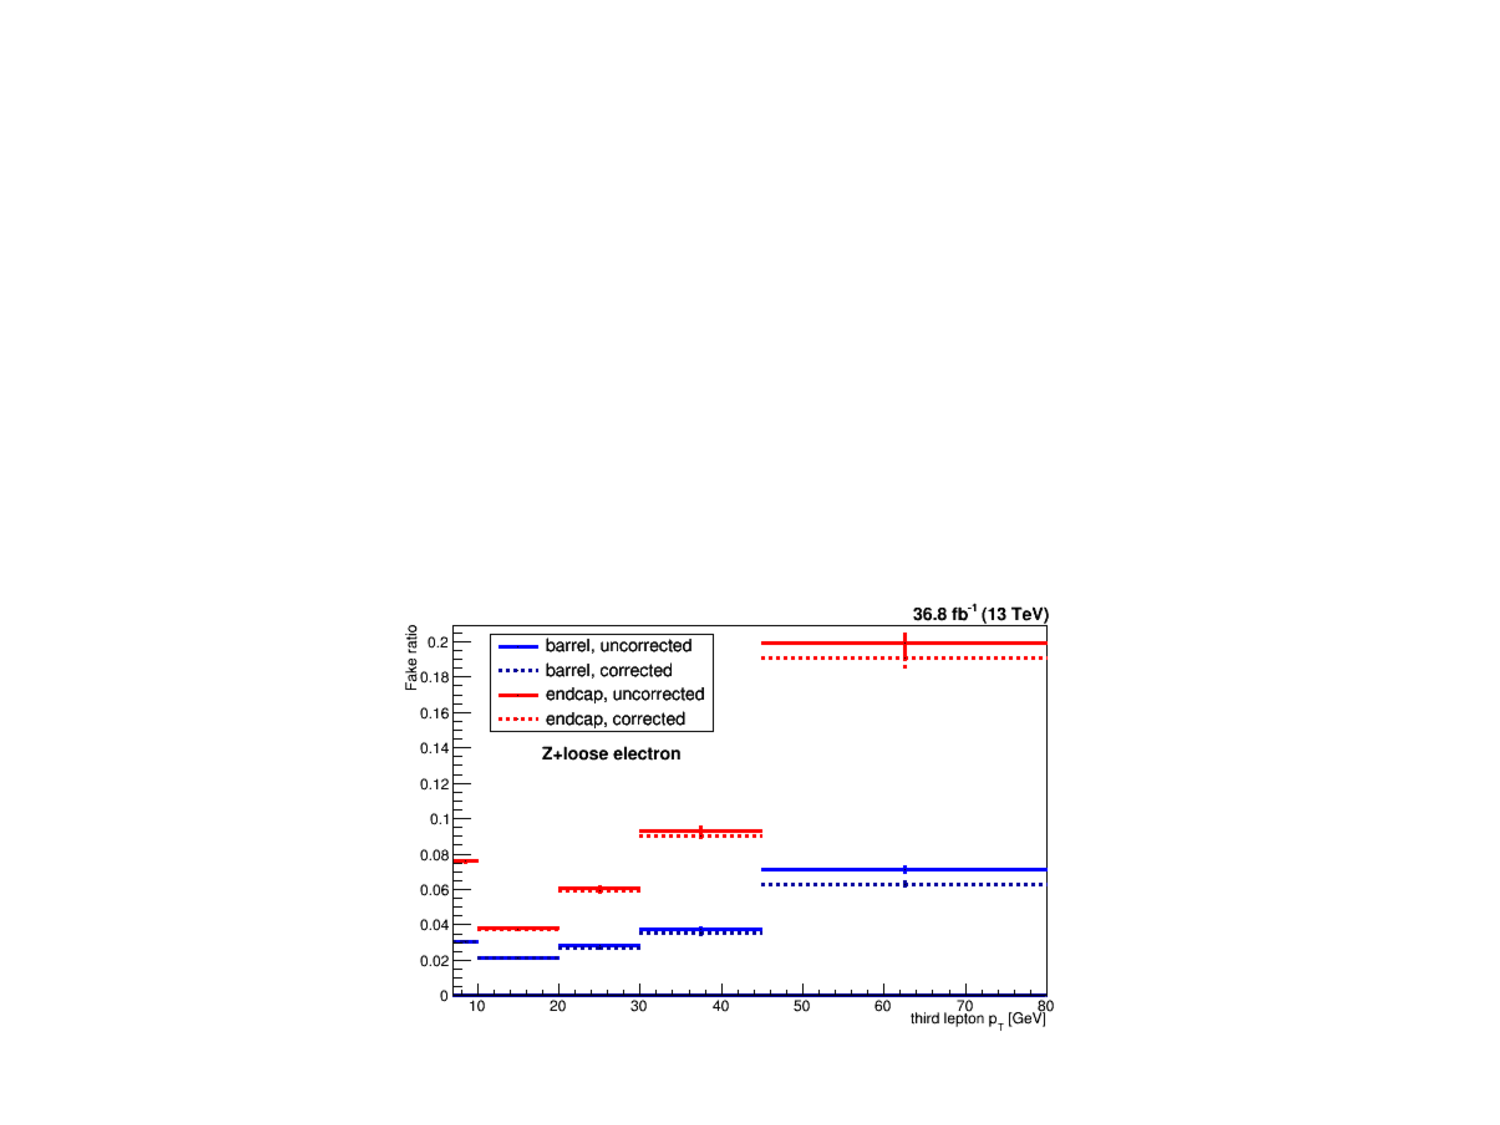
\includegraphics[width=4.25in]{Figures/RedBkg/FR_electrons_ptl3_DataallTR.pdf}
\caption{}
\end{subfigure}
\begin{subfigure}{0.95\textwidth}
\centering
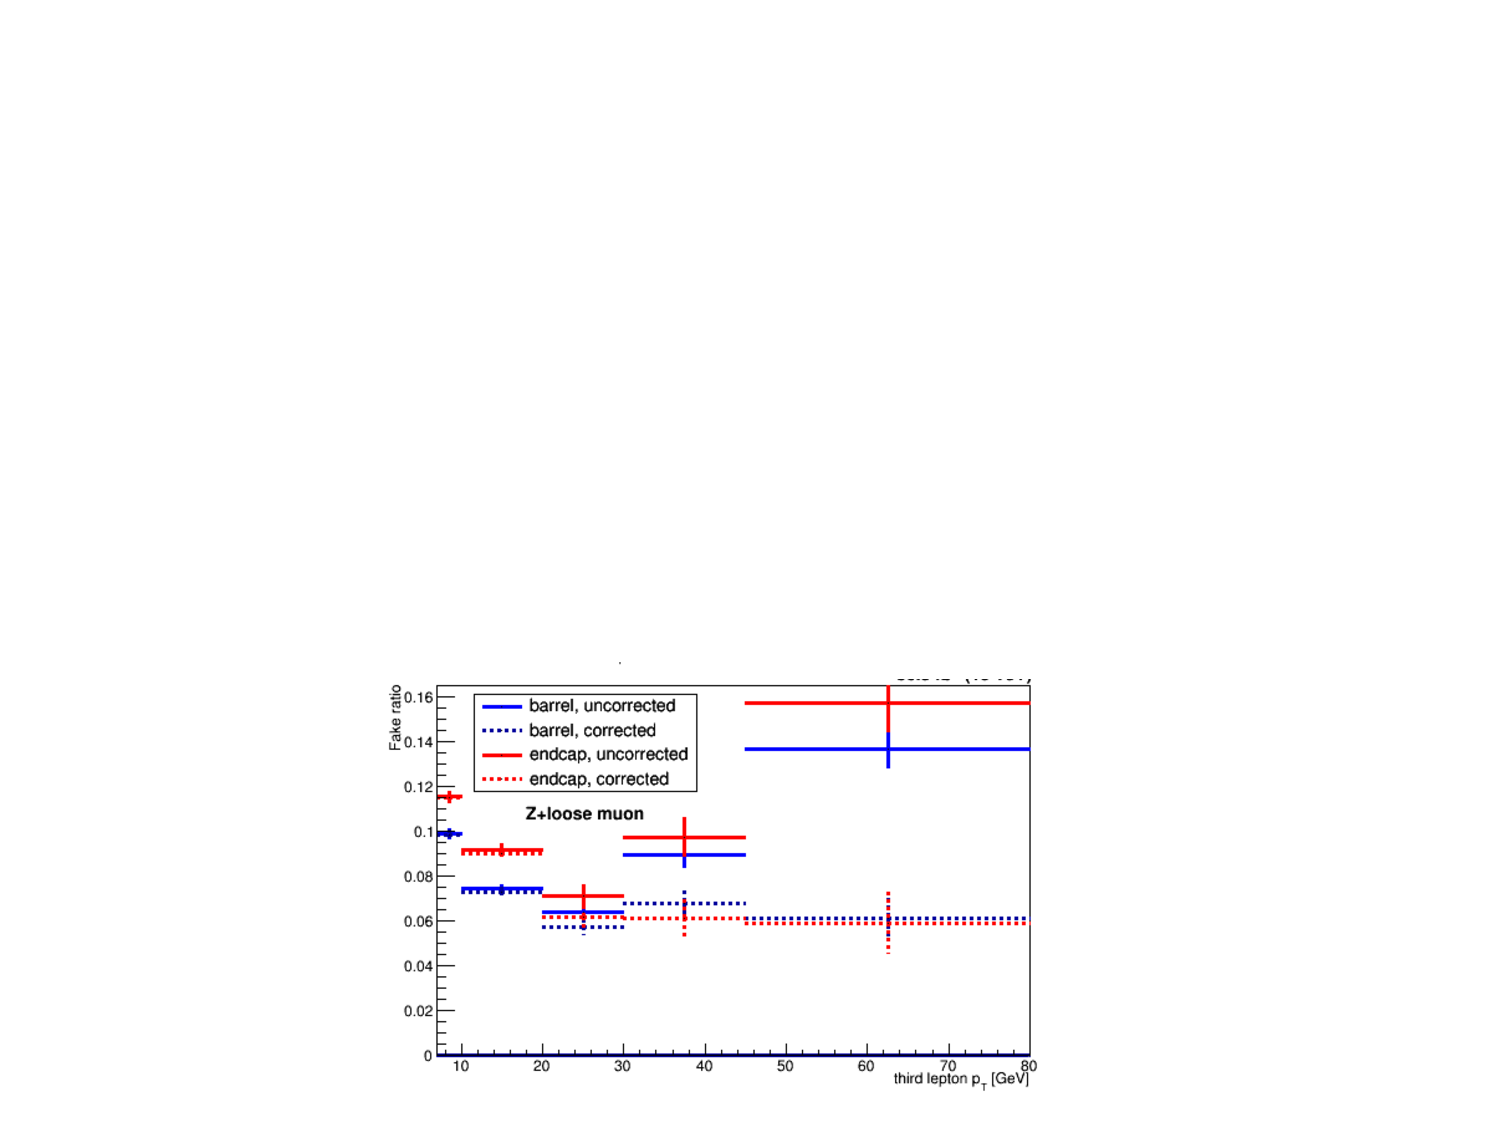
\includegraphics[width=4.25in]{Figures/RedBkg/FR_muons_ptl3_DataallTR.pdf}
\caption{}
\end{subfigure}
  \caption{
Fake rates as a function of the probe $p_T$ for electrons (a) and muons (b) which satisfy the loose selection criteria. The rake rates are measured in
a $Z(\ell\ell)+\ell$ sample in the $13$ $\TeV$ data.
The barrel selection includes electrons (muons) up to $|\eta|$ = 1.479 (1.2).
}
\label{fig:os_fakerates}
\end{figure}

%\begin{figure}[!htb]
%\begin{center}
%    \subfigure [] {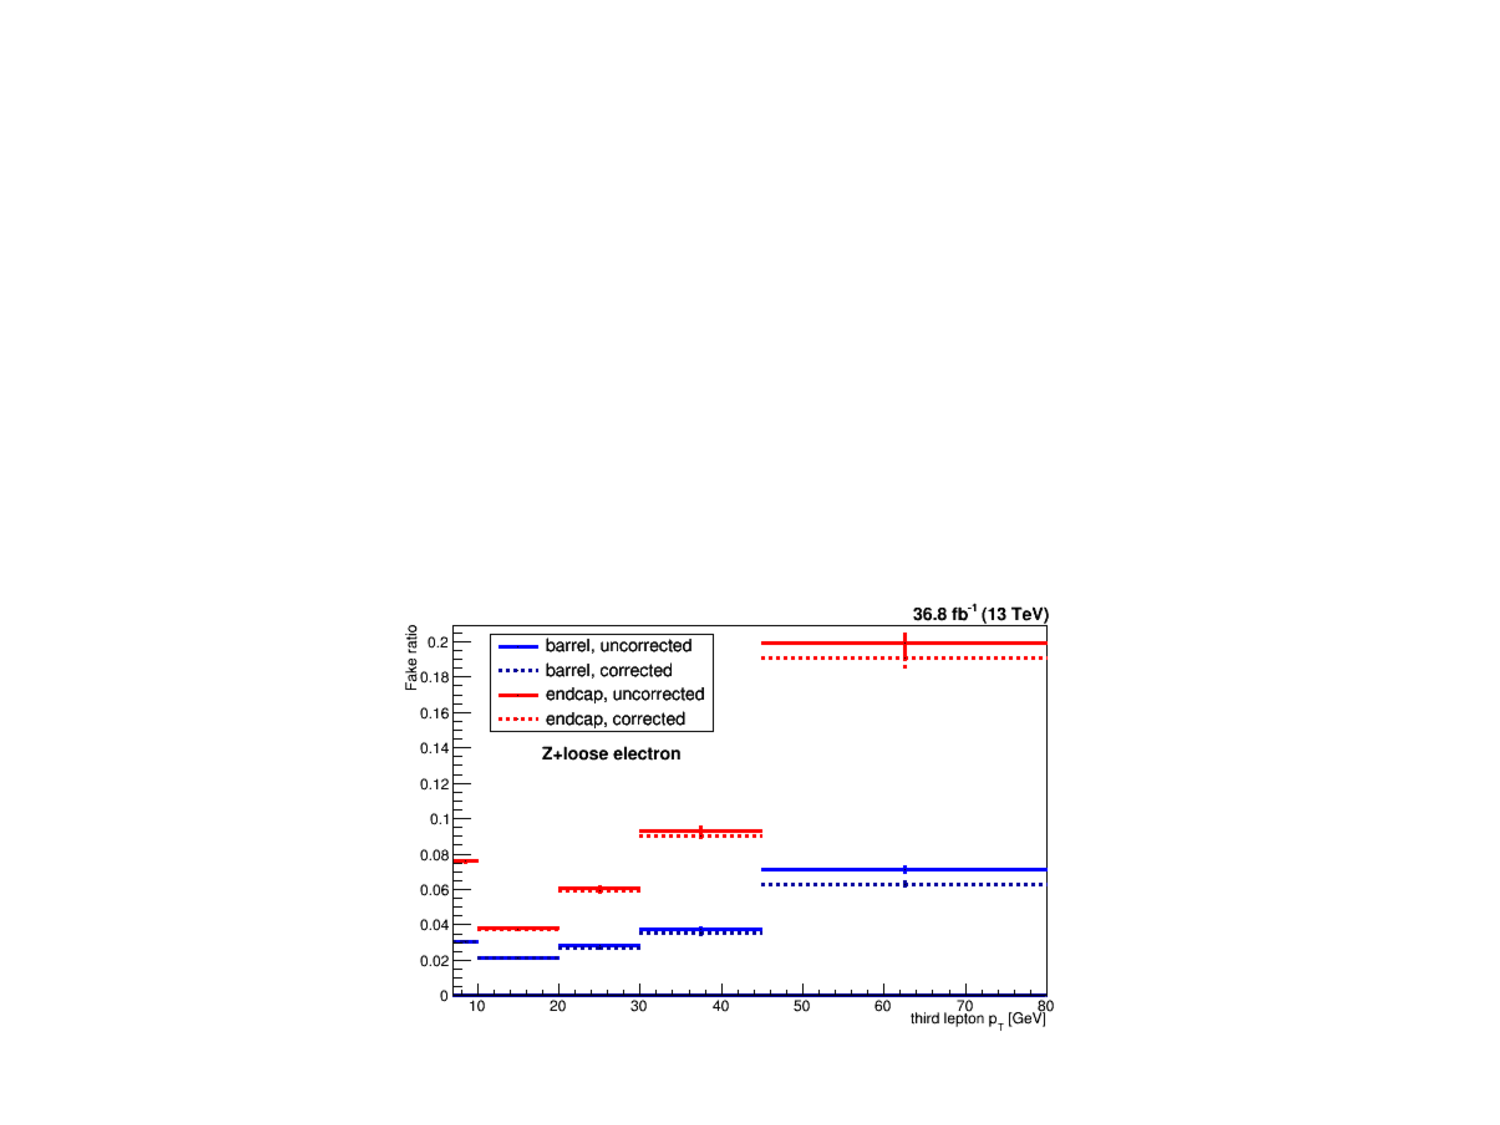
\includegraphics [width=0.45\textwidth]{Figures/RedBkg/FR_electrons_ptl3_DataallTR.pdf}}
%    \subfigure [] {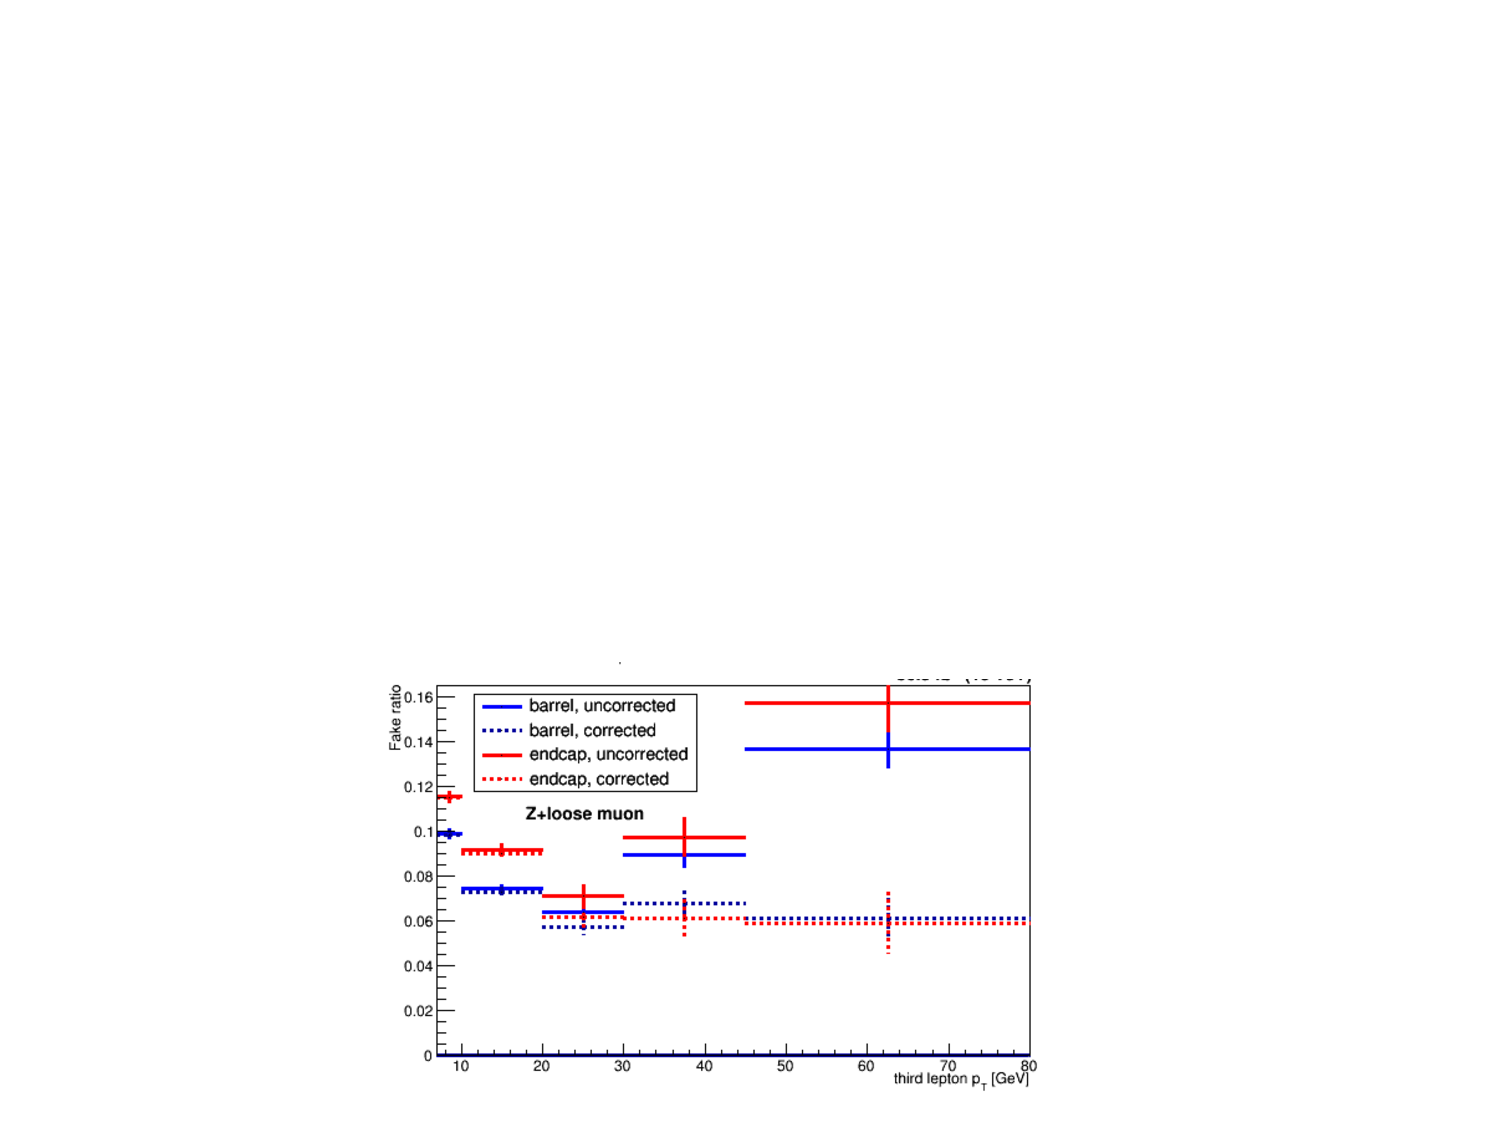
\includegraphics [width=0.45\textwidth]{Figures/RedBkg/FR_muons_ptl3_DataallTR.pdf}}
%  \caption{
%Fake rates as a function of the probe $p_T$ for  electrons (a) and muons (b) which satisfy the loose selection criteria, measured in
%a $Z(\ell\ell)+\ell$ sample in the $13$~TeV data.
%The barrel selection includes electrons (muons) up to $|\eta|$ = 1.479 (1.2).
%}
%\label{fig:os_fakerates}
%\end{center}
%\end{figure}



\subsubsection{Fake rate application}
\label{sec:zxA}

Two control regions are defined as subsets of four-lepton events
which pass the first step of the selection (see
Section~\ref{sec:zzcandsel}), requiring an additional pair of 
same-flavor, oppositely-charged loose leptons, that pass the ${\rm SIP_{3D}}$ cut. 
The events must satisfy all kinematic cuts applied for the Higgs phase space selection
(see Section~\ref{sec:zzcandsel}).
The first control sample is obtained by
requiring that the two loose leptons that do not make the $Z_1$ candidate 
do not pass the final identification and
isolation criteria.
The other two leptons pass
the final selection criteria by definition of the $Z_1$. 
This sample is denoted as the ``2 Prompt + 2
Fail'' (2P+2F) sample. It is expected to be populated with
events that intrinsically have only two prompt leptons, mostly $DY$, with a small fraction of $t \bar{t}$ and $Z \gamma$ events.
The second control sample is obtained by requiring one of
the four leptons not to pass the final identification and isolation
criteria.
The other three
leptons should pass the final selection criteria. This control sample
is denoted as ``3 Prompt + 1 Fail'' (3P+1F). It is
expected to be populated with the type of events that populate the
2P+2F region, 
albeit with different relative proportions,
as well as with $WZ$ events that intrinsically have three
prompt leptons.

The control samples obtained in this way, orthogonal by construction
to the SR, are enriched with fake leptons and are used to
estimate the reducible background in the SR. 

The invariant mass distribution of events selected in the 2P+2F control sample
is shown in Figure~\ref{fig:2P2F_dataMC} for the $13$ $\TeV$ dataset. 

\begin{figure}[!htb]
\begin{center}
    {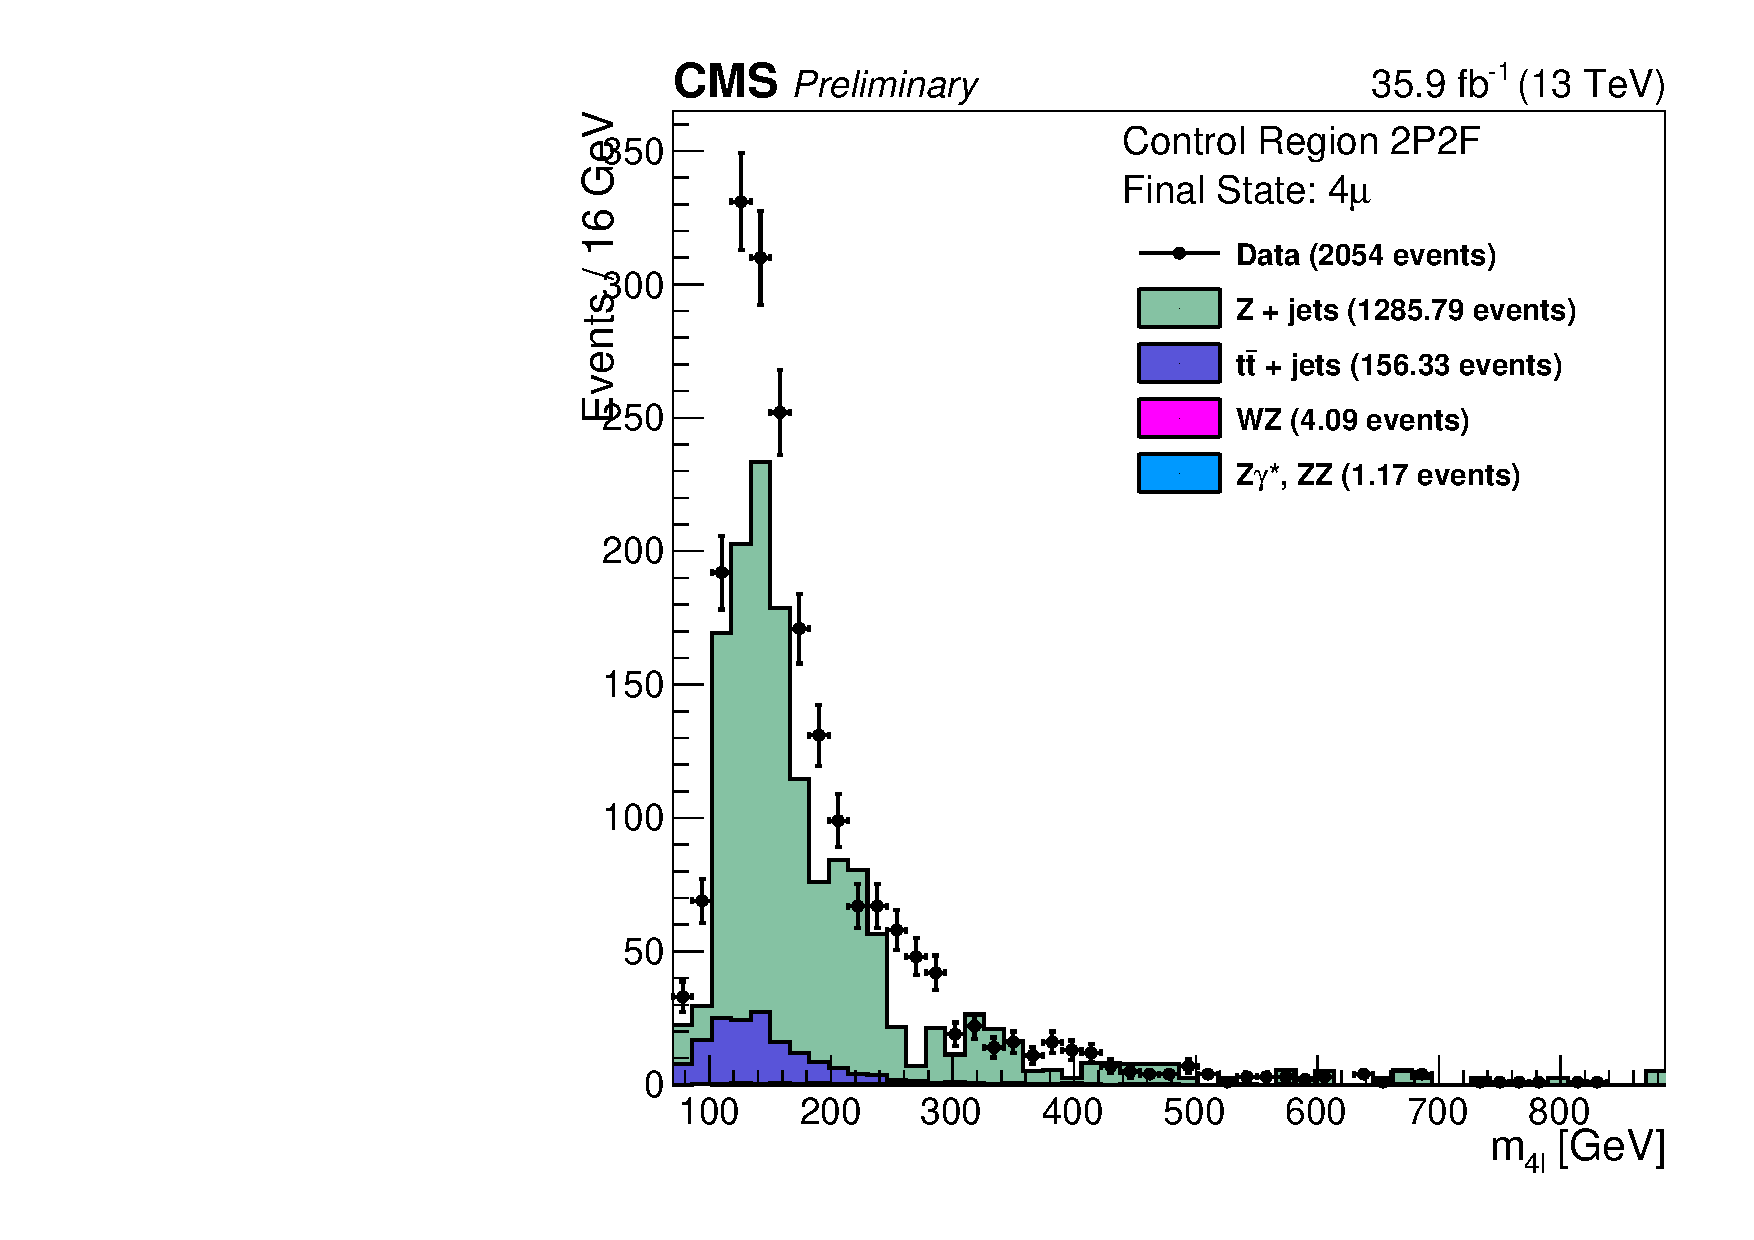
\includegraphics [width=0.45\textwidth] {Figures/RedBkg/HZZ_2P2Fuw_ZZMass_4m.pdf}}
    {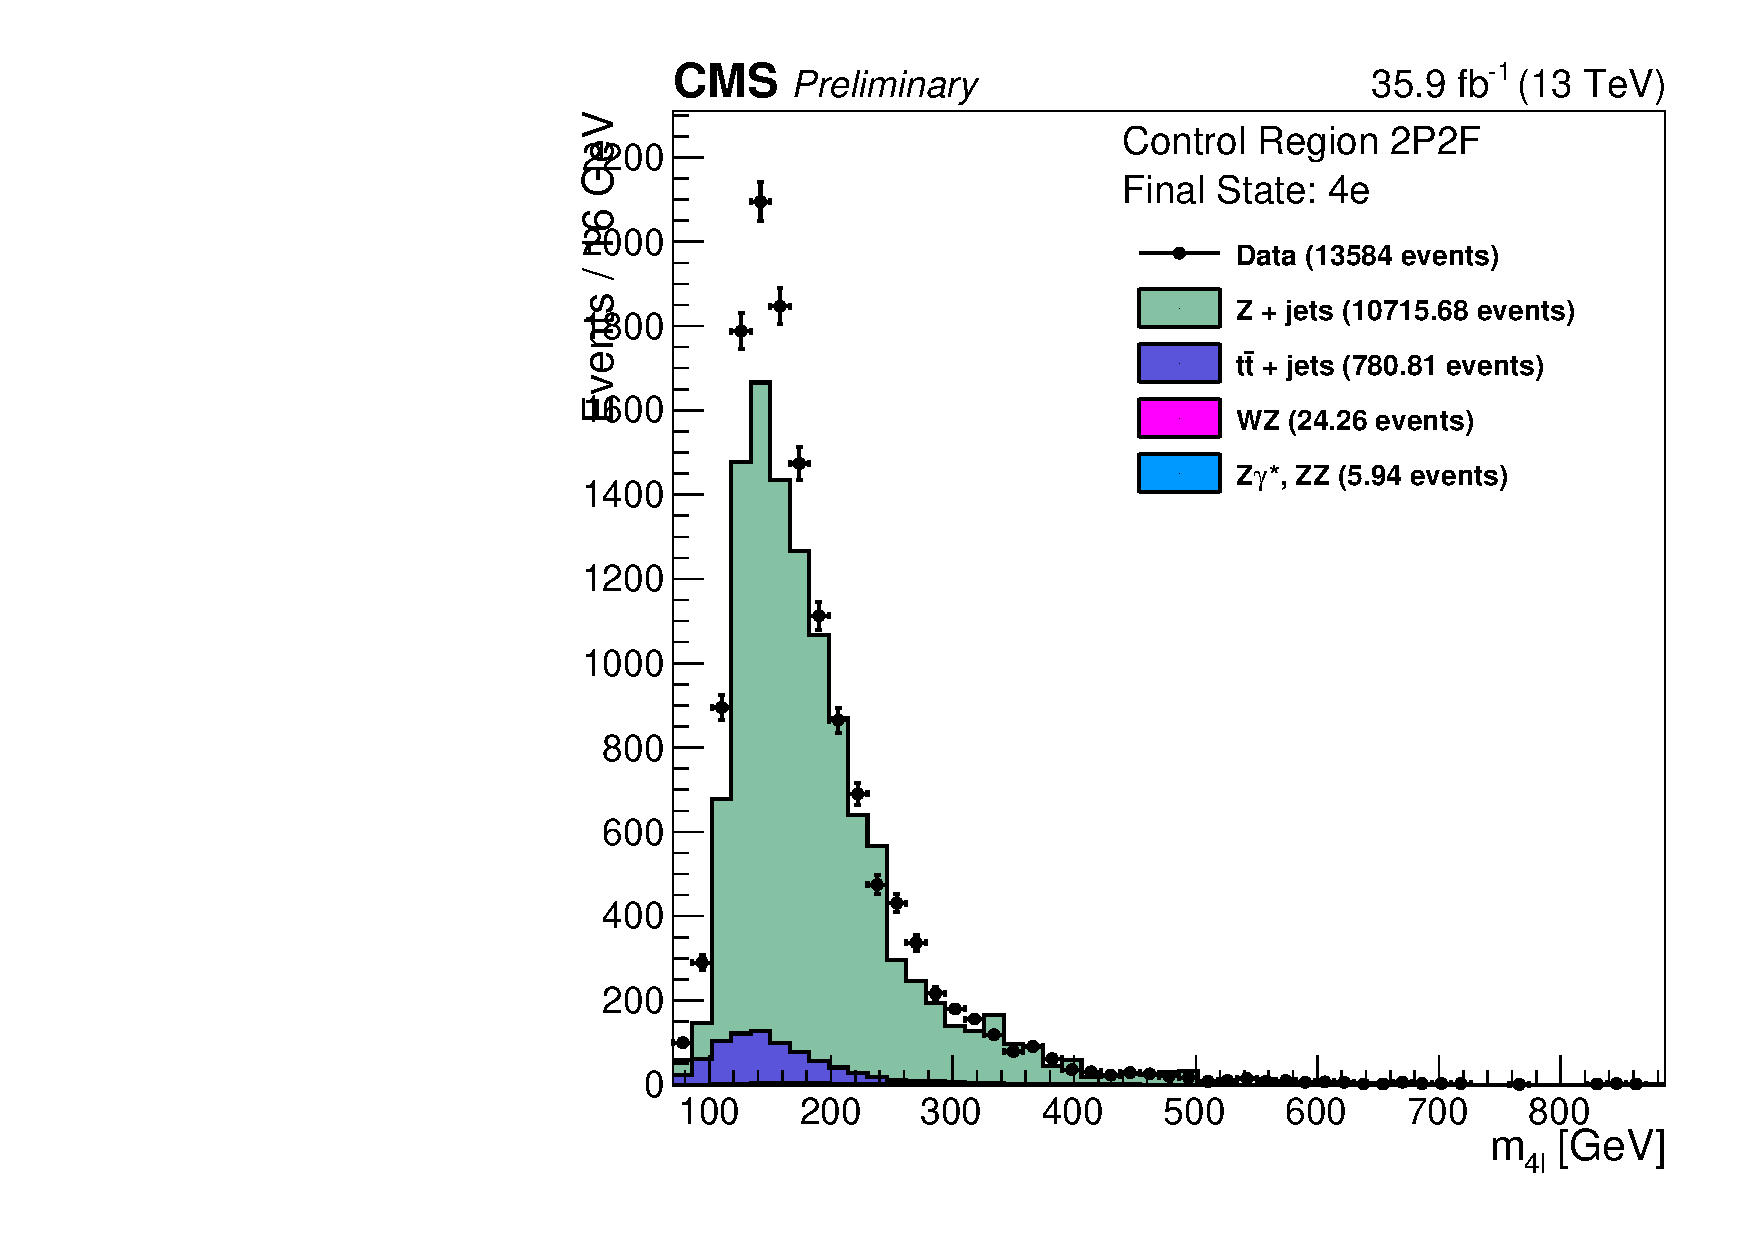
\includegraphics [width=0.45\textwidth] {Figures/RedBkg/HZZ_2P2Fuw_ZZMass_4e.pdf}} \\
    {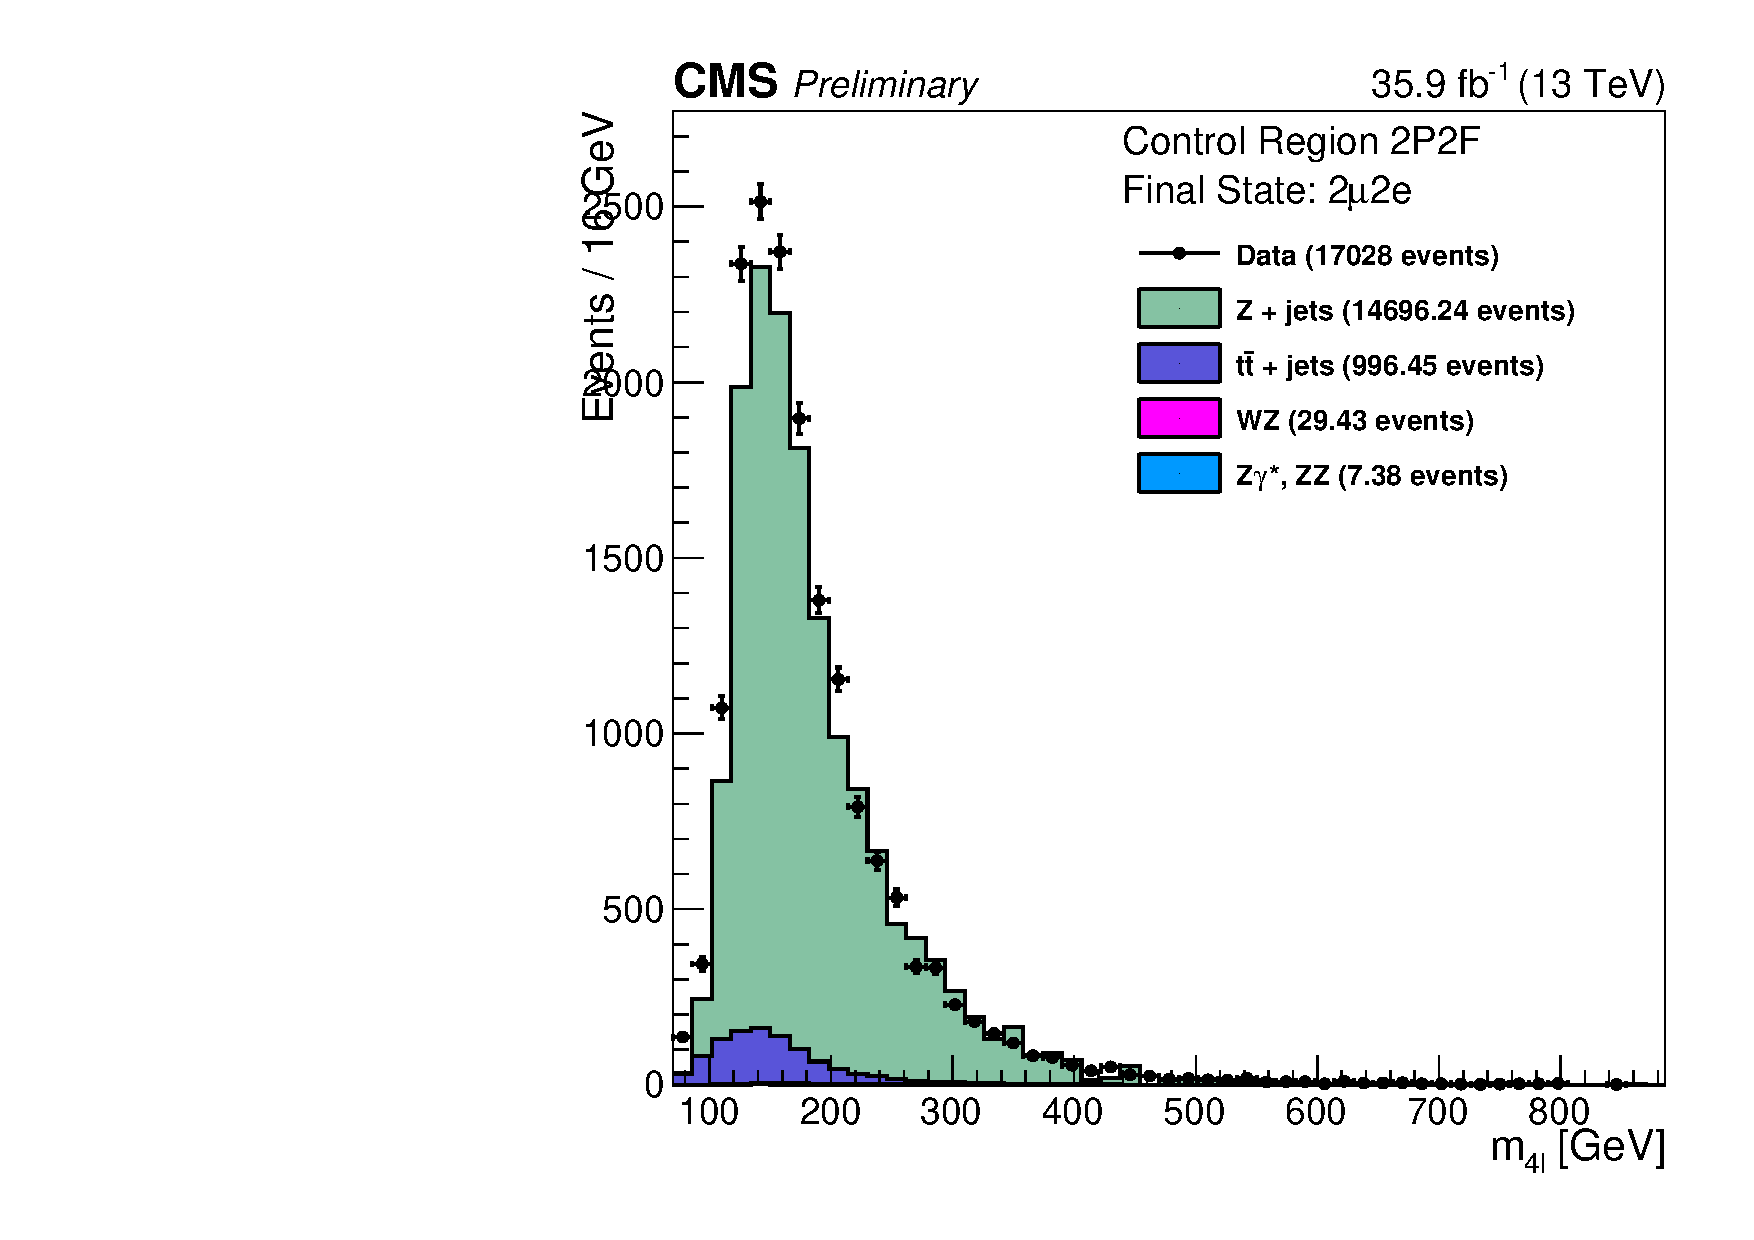
\includegraphics [width=0.45\textwidth] {Figures/RedBkg/HZZ_2P2Fuw_ZZMass_2m2e.pdf}}
    {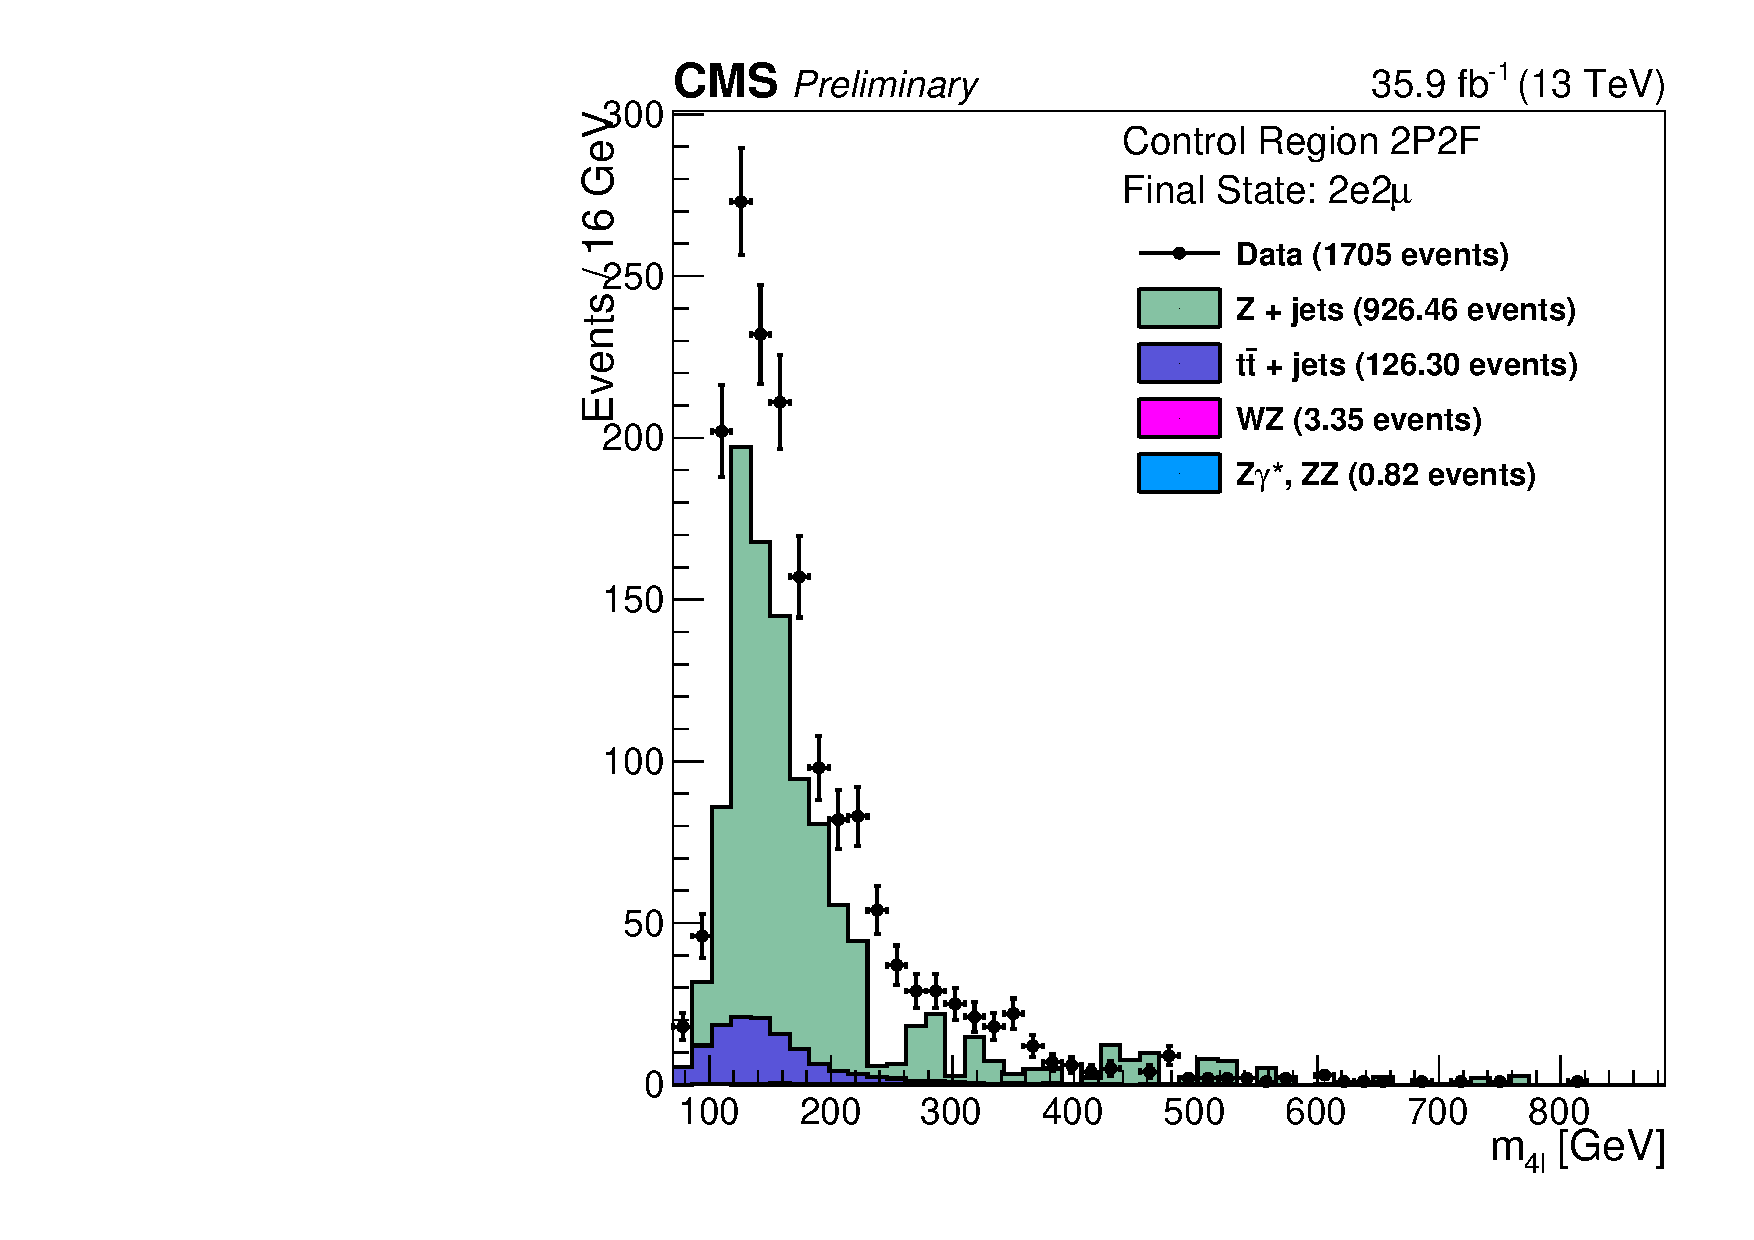
\includegraphics [width=0.45\textwidth] {Figures/RedBkg/HZZ_2P2Fuw_ZZMass_2e2m.pdf}} \\
\caption{
Invariant mass distribution of the events selected in the 2P+2F control sample in the
$13$ $\TeV$ dataset, (top left)  $4\mu$ , (top right) $4e$ , (bottom left)  $2\mu2e$ and (bottom right)  $2e2\mu$ channels.
}
\label{fig:2P2F_dataMC}
\end{center}
\end{figure}

\begin{figure}[!htb]
\begin{center}
    {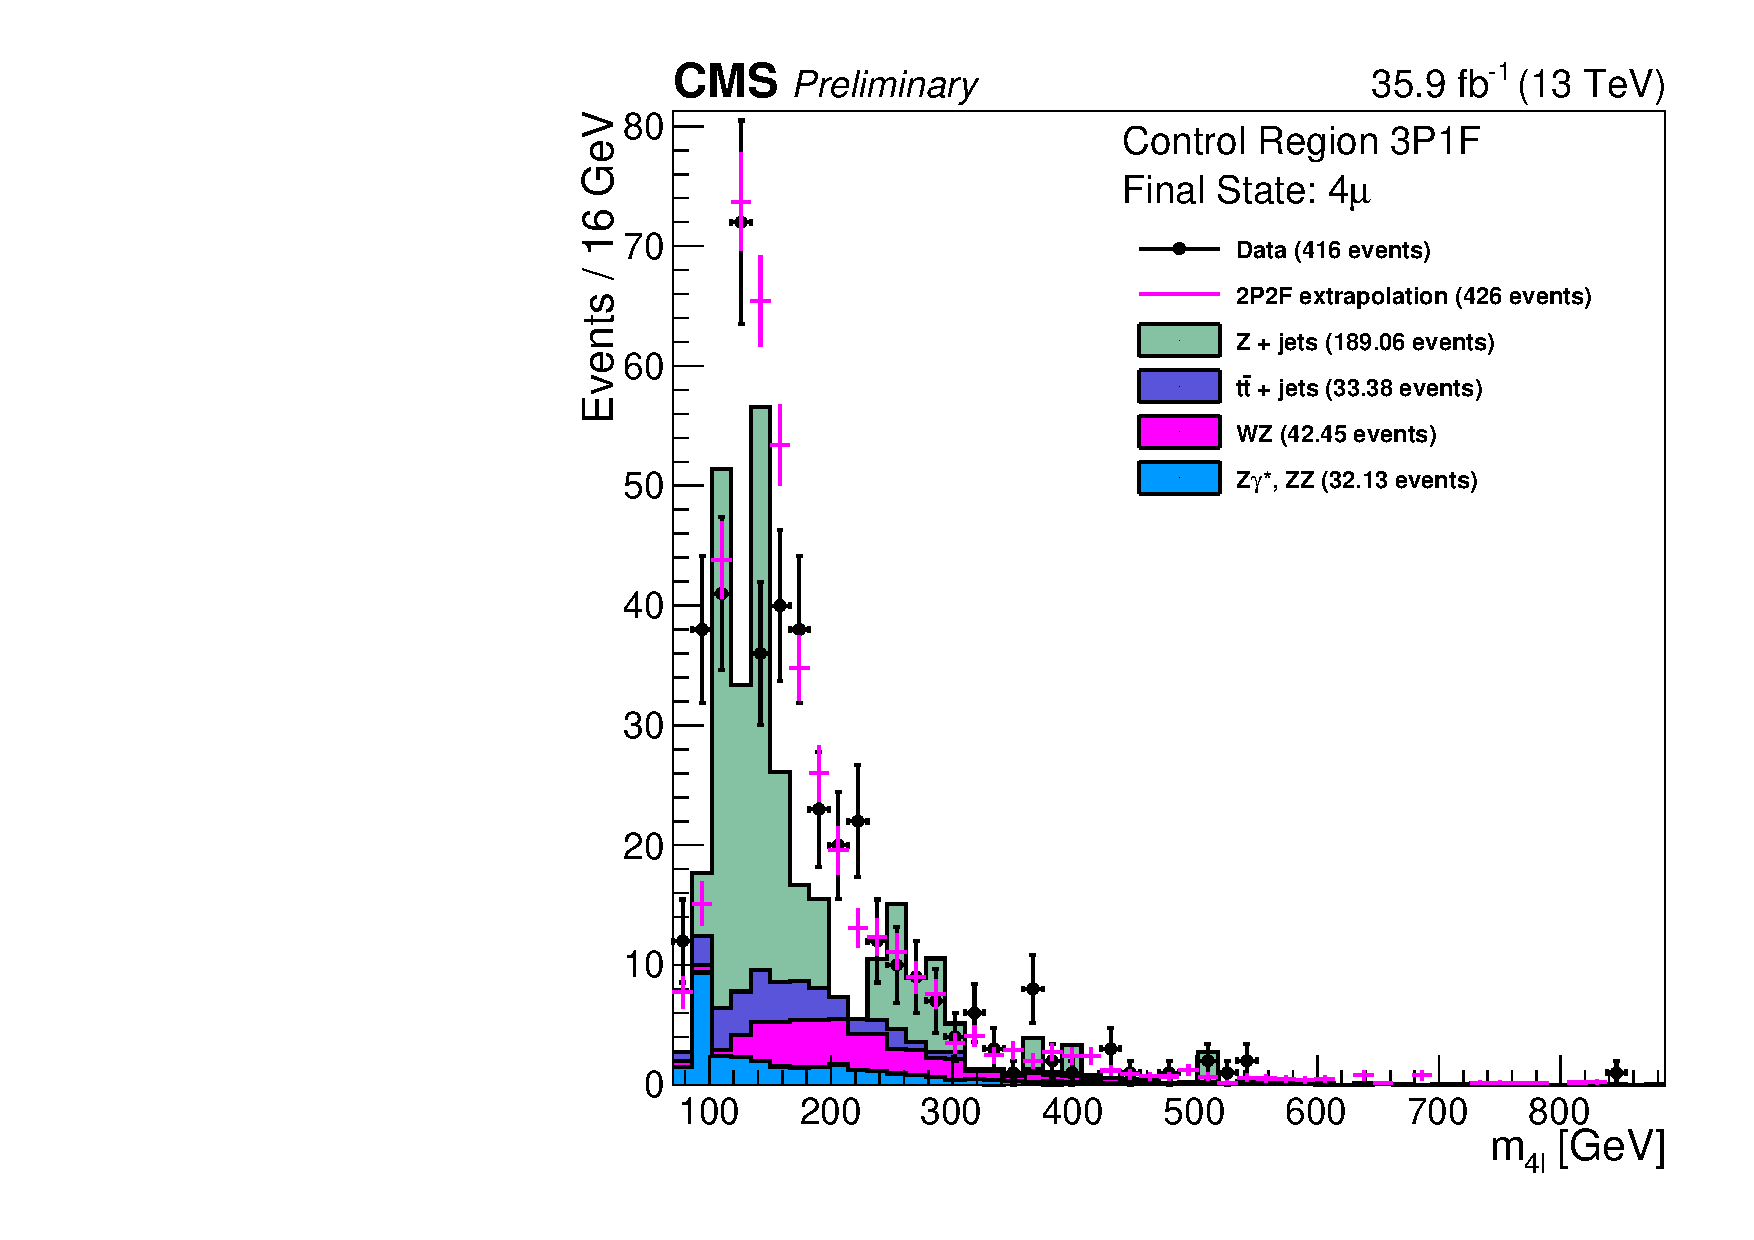
\includegraphics [width=0.45\textwidth] {Figures/RedBkg/HZZ_3P1Fuw_ZZMass_4m.pdf}}
    {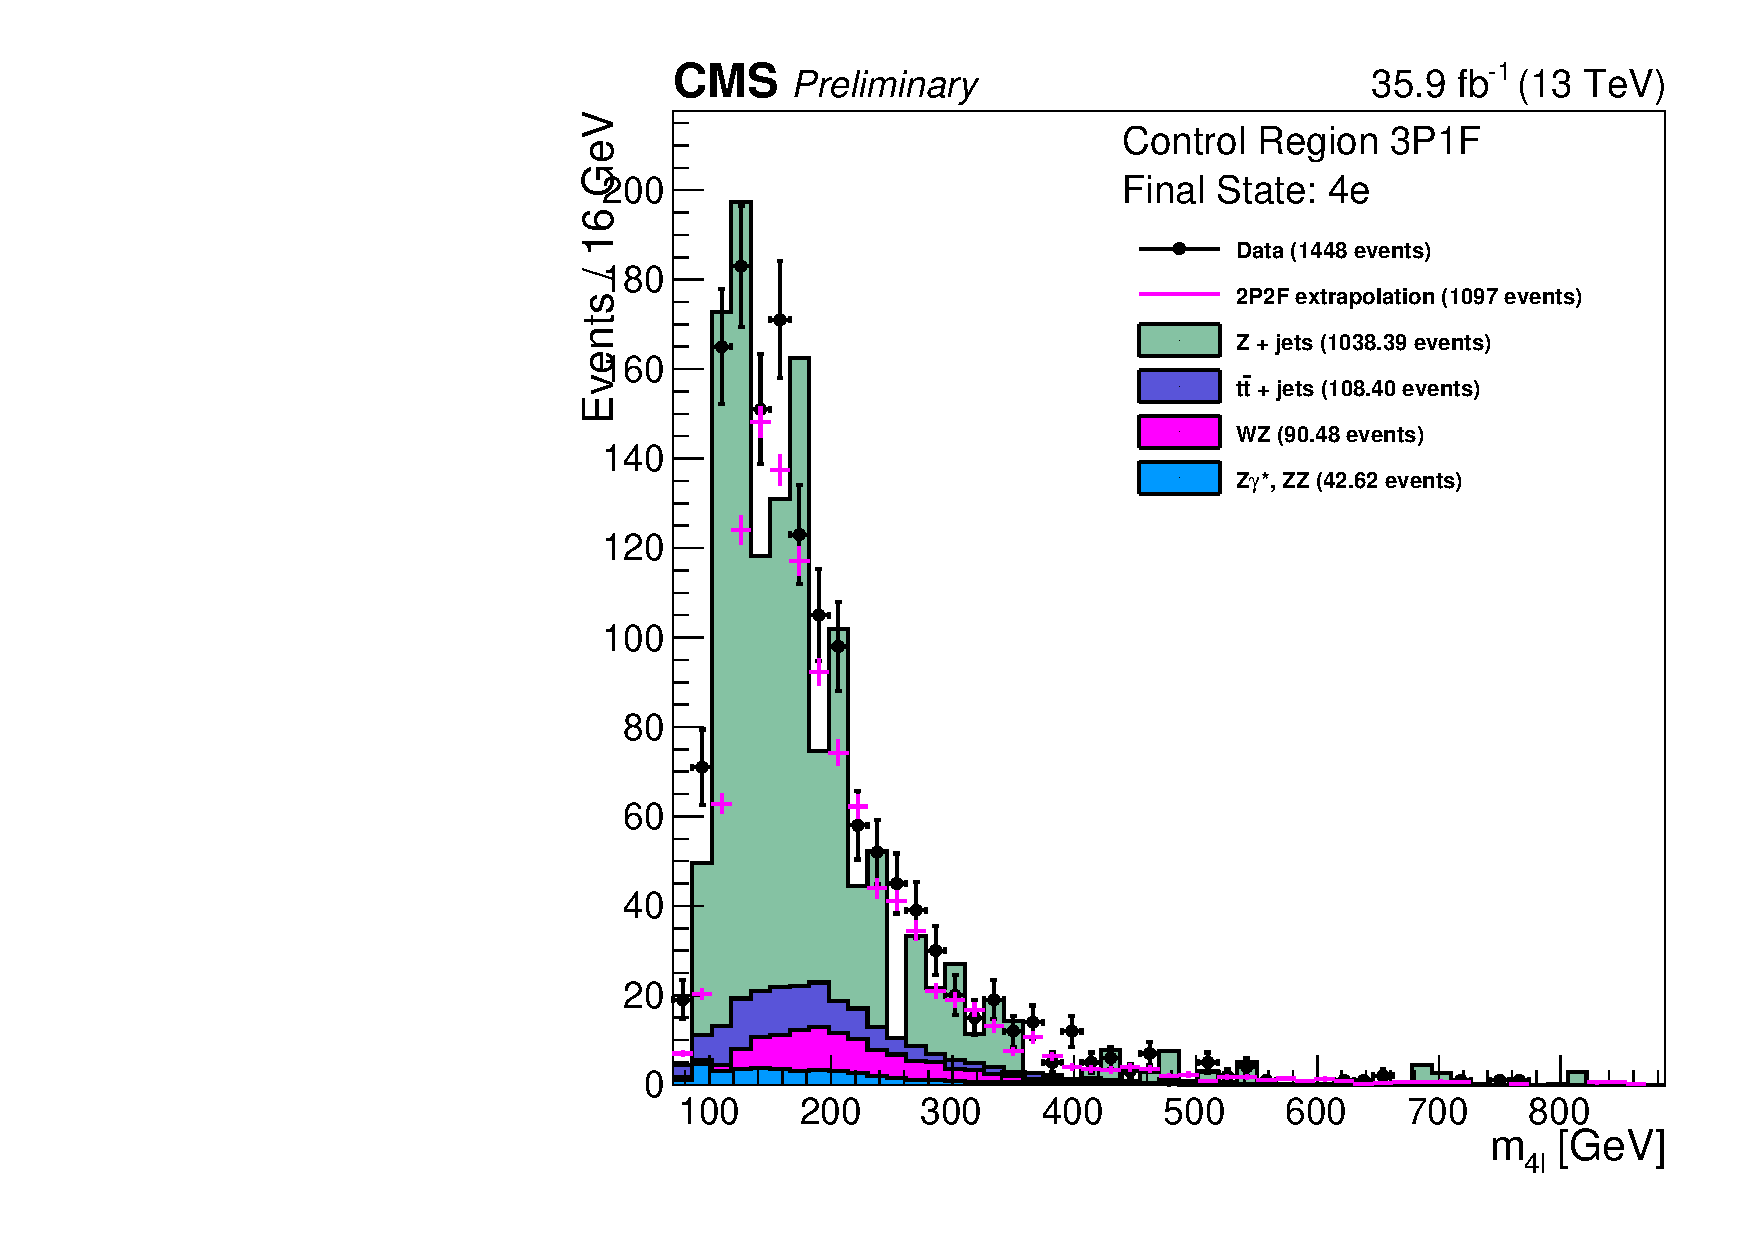
\includegraphics [width=0.45\textwidth] {Figures/RedBkg/HZZ_3P1Fuw_ZZMass_4e.pdf}} \\
    {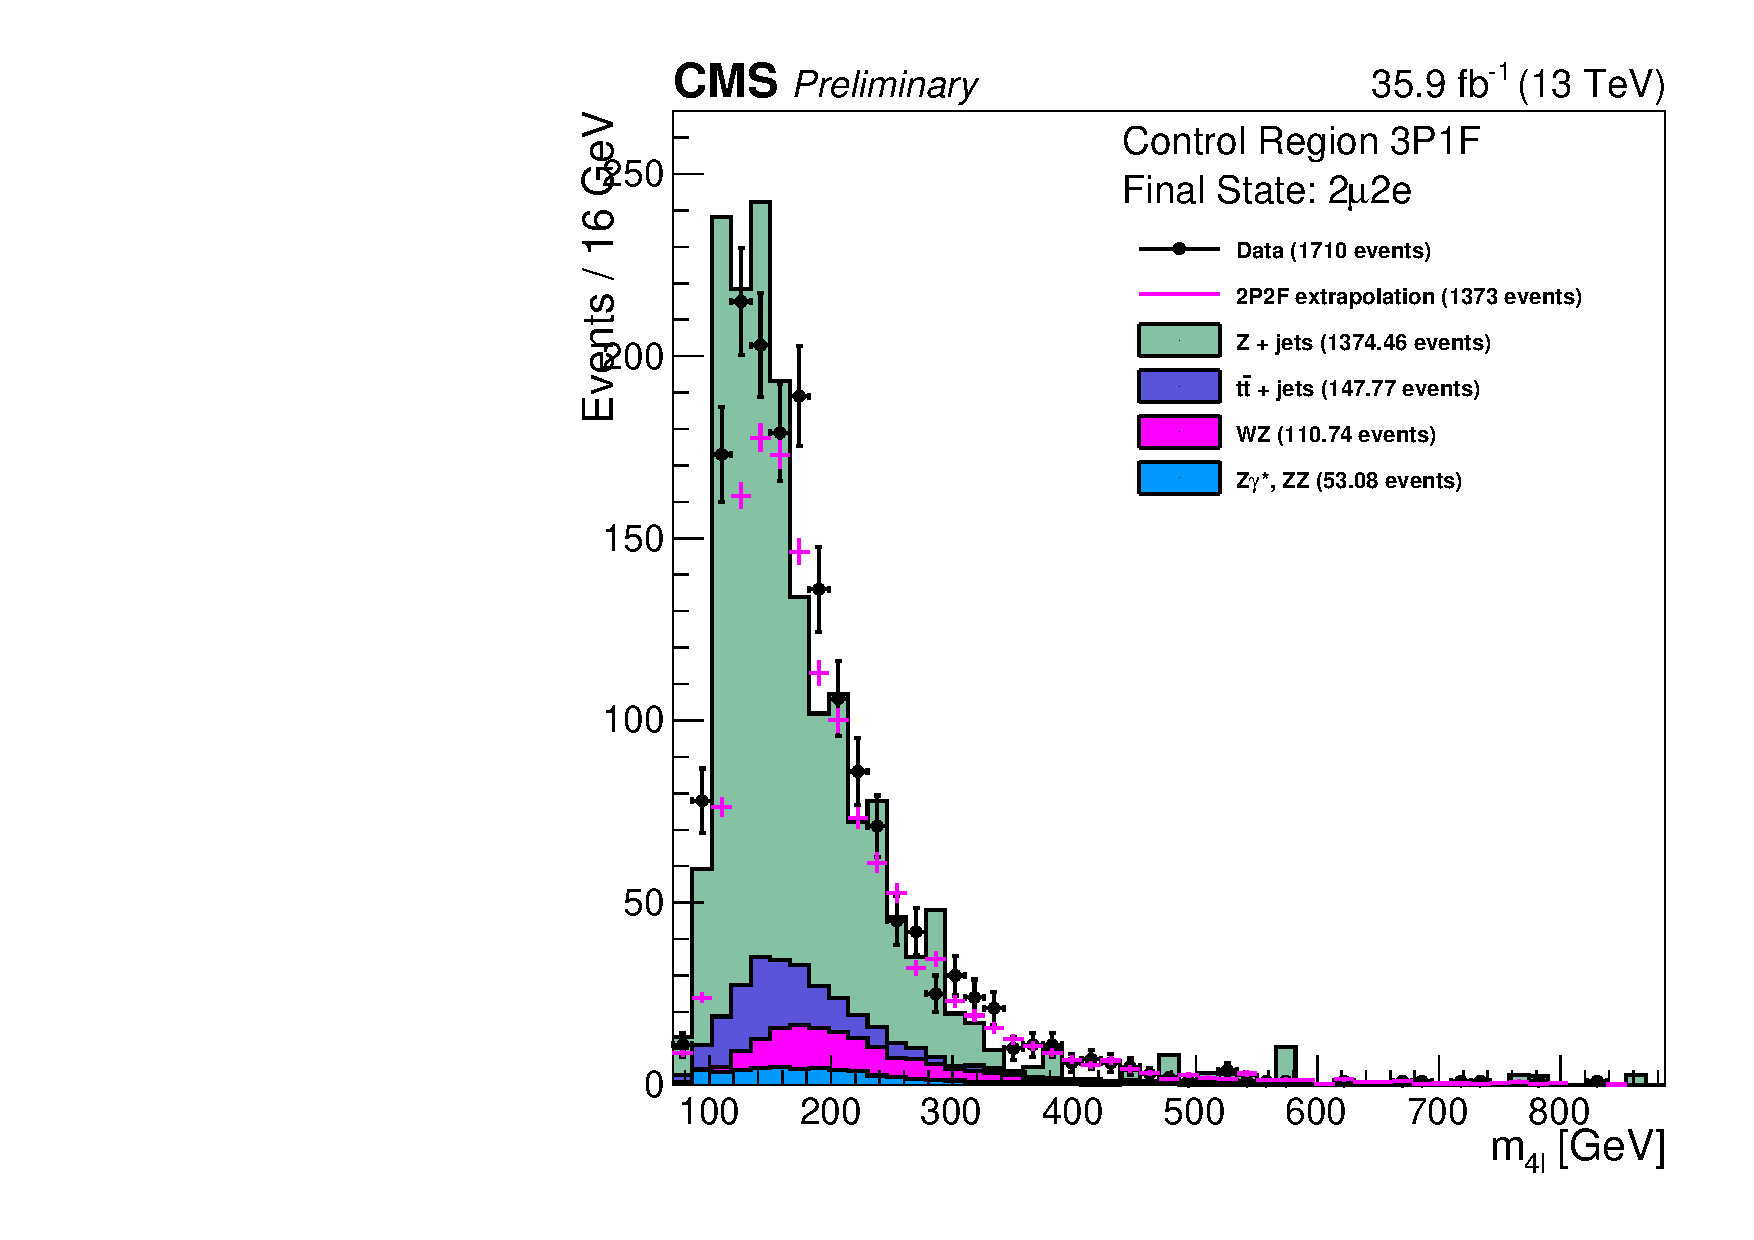
\includegraphics [width=0.45\textwidth] {Figures/RedBkg/HZZ_3P1Fuw_ZZMass_2m2e.pdf}}
    {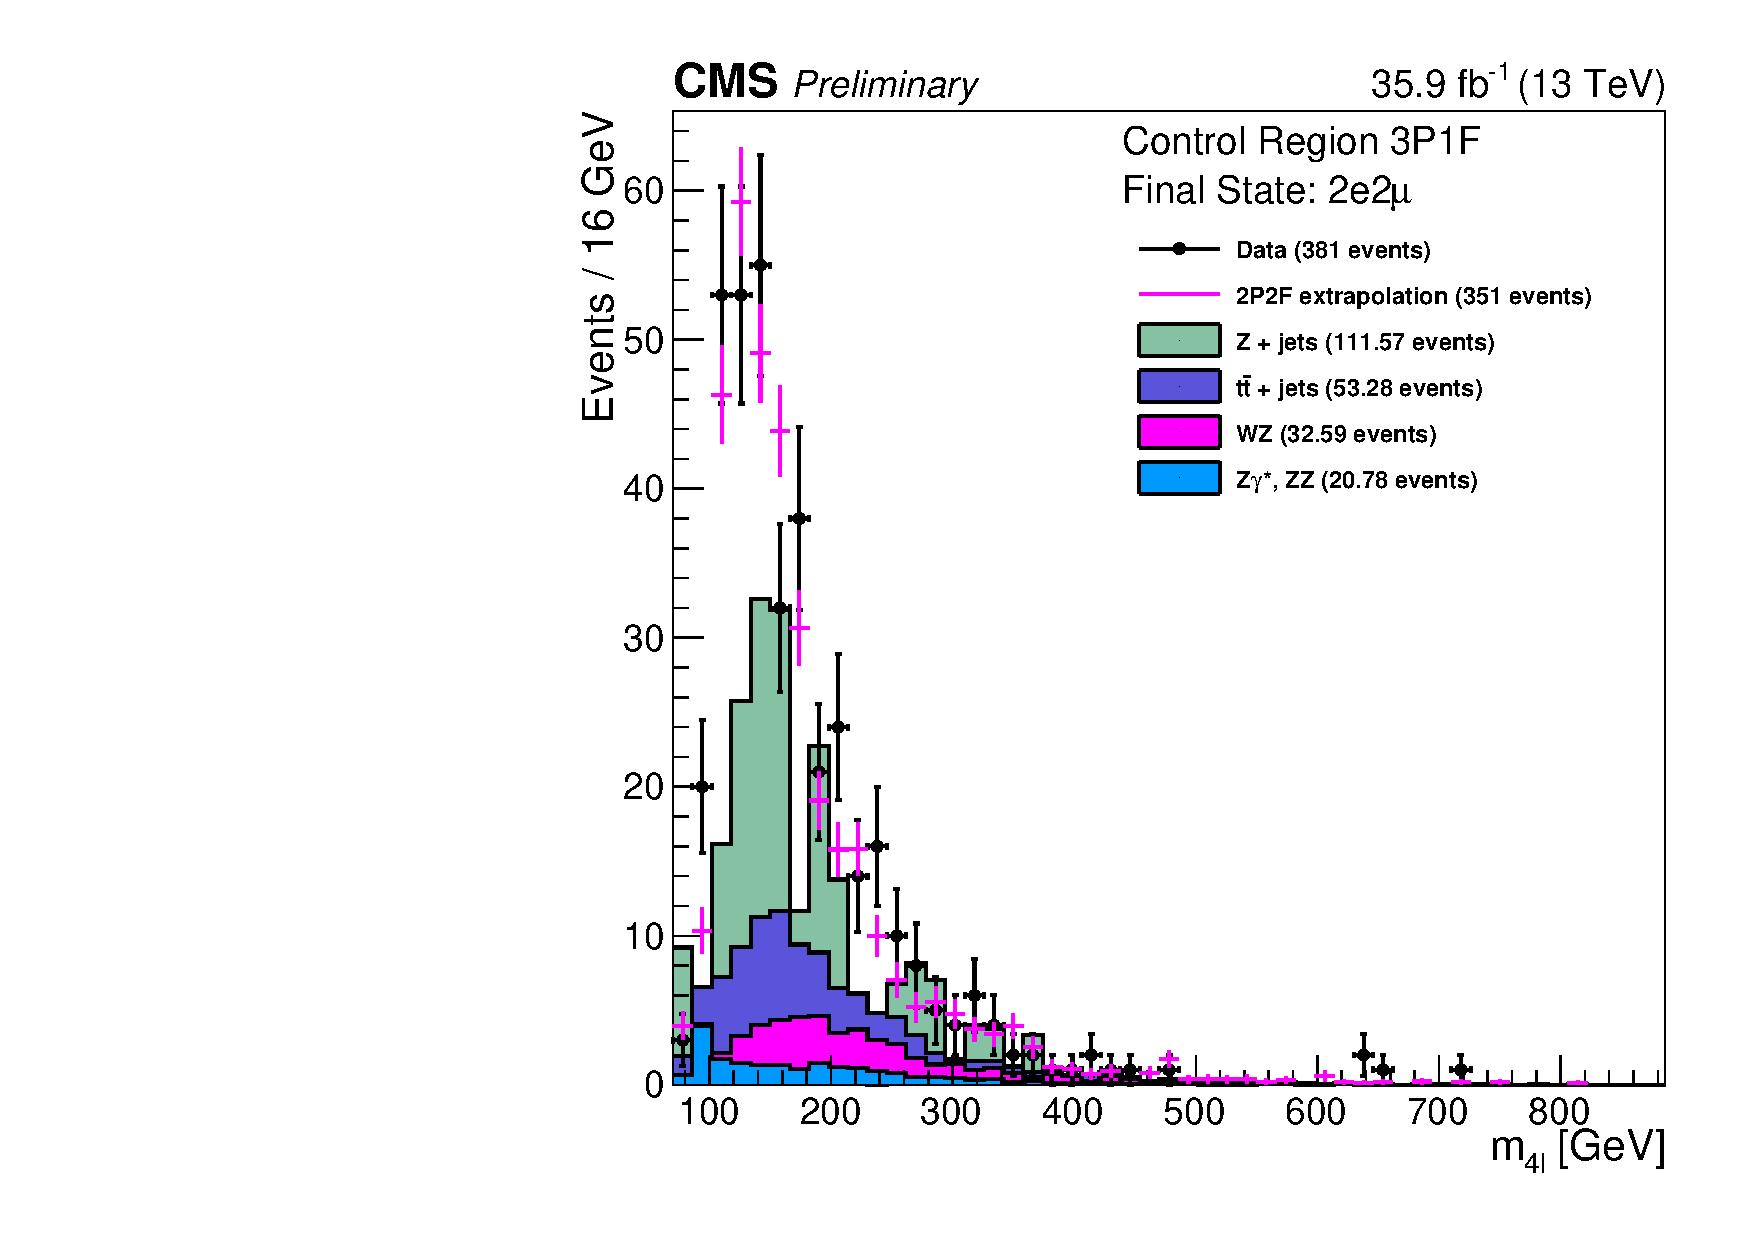
\includegraphics [width=0.45\textwidth] {Figures/RedBkg/HZZ_3P1Fuw_ZZMass_2e2m.pdf}} \\
\caption{
Invariant mass distribution of the events selected in the 3P+1F control sample in the
$13$ $\TeV$ dataset, (top left)  $4\mu$ , (top right) $4e$ , (bottom left)  $2\mu2e$ and (bottom right)  $2e2\mu$ channels.
}
\label{fig:CR_3P1F}
\end{center}
\end{figure}

The expected number of reducible background events in the 3P+1F region,
$N^{\rm bkg}_{\rm 3P1F}$, can be computed from the number of events
observed in the 2P+2F control region, $N_{\rm 2P2F}$, by weighting each
event in the region with the factor $(\frac{f_{i}}{1-f_{i}}
+ \frac{f_{j}}{1-f_{j}})$, where $f_{i}$ and $f_{j}$ correspond to the
fake rates of the two loose leptons:

\begin{equation} 
\label{eq:Prediction3P1F}
N^{\rm bkg}_{\rm 3P1F} = \sum (\frac{f_{i}}{1-f_{i}}
+ \frac{f_{j}}{1-f_{j}}) N_{\rm 2P2F}
\end{equation} 

Figure~\ref{fig:CR_3P1F} shows the invariant mass distributions of the
events selected in the 3P+1F control sample, together with the expected
reducible background estimated from Equation~\ref{eq:Prediction3P1F},
stacked on the distribution
of $WZ$ and of irreducible background ($ZZ, Z\gamma* \to 4\ell$) taken from simulation.

If the fake rates were measured in a sample that had exactly the same
background composition as the 2P+2F sample, the difference between the
observed number of events in the 3P+1F sample and the expected background
predicted from the 2P+2F sample would solely amount to the $WZ$ and $Z\gamma_{conv}$
contribution, which is small. Large differences arise because the fake rates used in
Equation~\ref{eq:Prediction3P1F} do not properly account for the background
composition of the 2P+2F control sample.

The difference seen in Figure~\ref{fig:CR_3P1F} between the observed
3P+1F distribution and the expectation from 2P+2F in the
channels with loose electrons ($4e$ and $2\mu 2e$), concentrated at low
masses, is due to photon conversions. This is confirmed explicitly by simulation.
% : Fig.~\ref{fig:CR_3P1F}c shows how events with a real photon populate
% this low mass region. Indeed, as the fake rates of method A are measured
% in a sample that is largely devoid of photon conversions, Eq.~\ref{eq:Prediction3P1F}
% considerably underestimates their contribution to the 3P+1F sample. 
%
The difference between the 3P+1F observation and the prediction
from 2P+2F is corrected to recover the missing contribution from conversions.
More precisely, the expected reducible background in the SR is given
by the sum of two terms: a 2P2F component and a 3P1F component.

The 2P2F component is obtained from the number of
  events observed in the 2P+2F control region, $N_{\rm 2P2F}$, by
  weighting each event in that region with the factor
  $\frac{f_{i}}{1-f_{i}} \frac{f_{j}}{1-f_{j}}$, where $f_{i}$ and
  $f_{j}$ correspond to the fake rates of the two loose leptons.
The 3P1F component is obtained from the
   difference between the number of observed events in the 3P+1F control
   region, $N_{\rm 3P1F}$, and the expected contribution from the 2P+2F
   region and $ZZ$ processes in the signal region, $N^{\rm ZZ}_{\rm 3P1F} +
   N^{\rm bkg}_{\rm 3P1F}$. The $N^{\rm bkg}_{\rm 3P1F}$ is given by 
   Equation~\ref{eq:Prediction3P1F} and $N^{\rm ZZ}_{\rm 3P1F}$ is the
   contribution from $ZZ$ which is taken from simulation. 
   The difference $N_{\rm 3P1F} -  N^{\rm bkg}_{\rm 3P1F} - N^{\rm ZZ}_{\rm 3P1F}$,
   which may be negative,
   is obtained for each $(p_T, \eta)$ bin of the probe lepton and is weighted 
   by $\frac{f_i} {1 - f_i}$, where $f_i$ denotes the fake rate of
   this lepton.
   This 3P1F component accounts for the contribution of reducible background
   processes with only one fake lepton (like $WZ$ events) and for the contribution
   of other processes (e.g. photon conversions) that are not properly estimated
   by the 2P2F component because of the fake rates used.

The full expression for the prediction can be symbolically written as:
%
\begin{equation} 
\label{eq:PredictionSR}
N^{bkg}_{\rm SR} = \sum \frac{f_{i}}{(1-f_{i})} (N_{\rm 3P1F} - N^{\rm
bkg}_{\rm 3P1F} - N^{\rm ZZ}_{\rm 3P1F})
+ \sum \frac{f_{i}}{(1-f_{i})} \frac{f_{j}}{(1-f_{j})}N_{\rm 2P2F} \end{equation}
%a
or equivalently:
\begin{equation}
\label{eq:PredictionSR2}
N^{bkg}_{\rm SR}= (1-\frac{N_{3P1F}^{ZZ}}{N_{3P1F}})\sum_j^{N_{3P1F}}\frac{f_a^j}{1-f_a^j} - \sum_i^{N_{2P2F}}\frac{f_3^i}{1-f_3^i}\frac{f_4^i}{1-f_4^i}
\end{equation}
For channels where the $Z_2$ candidate is made from two electrons, 
the contribution of the 3P1F component is 
positive and amounts to typically $30 \%$ of the total predicted background.

For channels with loose muons (e.g. $\mu$ and $2e2\mu$), the 3P+1F sample is rather well described by
the prediction from 2P+2F, as seen in Figure~\ref{fig:CR_3P1F}, and the
3P1F component is mainly driven by statistical fluctuations in the 3P+1F sample,
which are larger than the expectation from $WZ$ production.


Table~\ref{tab:reducibleMethodA} shows the expected number of
events in the four-lepton SRs from the reducible background processes. 
% The first error is the statistical uncertainty, which is dominated by the
% large statistical uncertainty of the ``3P1F" component. The second error
% is a systematic uncertainty due to the statistical uncertainty of the
% fake rates.

\begin{table}[h]
\begin{center}
     \begin{tabular}{| l | c | c | c | c |} \hline
 baseline	& $4e$ 	 & 4$\mu$ & $2e2\mu$  & 2$\mu2e$   \\ \hline \hline
 13 $\TeV$		& $22.19$ & $32.81$ & $22.48$    & $41.72$  \\  \hline
 	\end{tabular}
\end{center}
    \caption{ The contribution of reducible background
    processes in the four-lepton signal region predicted from measurements in data
    using the Opposite-Sign Leptons method. The predictions correspond to \usedLumi of data at 13 $\TeV$.}
     \label{tab:reducibleMethodA}
\end{table}


\section{Event yields}

Table~\ref{tab:smyields} shows the event yields for the primary backgrounds, a benchmark signal, and the observed events at the major event selection stages. This is called the analysis cutflow. The selection of tight leptons and the formation of the first $Z$ candidate are sufficient to remove most of the background events. After the second $Z$ is formed, the remaining selection steps do not reduce backgrounds significantly but assist in the selection of events with clean $ZZ^*$ candidates. 

\begin{table*}[htbH]
\begin{center}
\resizebox{\textwidth}{!}{%
\begin{tabular}{ l | c | c | c | c | c | c | c | c }
\hline
\hline
Sample & $q\bar{q} \rightarrow ZZ$ & $gg \rightarrow ZZ$ & $Z+X$ & $ZH$ & Other $H$ & Total & Signal & Observed \\
\hline
Initial & 1.89e+04 & 866 & 5.88e+08 & 17.4 & 377 & 5.88e+08 & 3.57 & 8.21e+07 \\
\hline
HLT & 1.89e+04 & 866 & 5.88e+08 & 17.4 & 377 & 5.88e+08 & 3.57 & 8.21e+07 \\
\hline
$Z_1$ lepton cuts & 1.94e+03 & 144 & 5.9e+04 & 2.35 & 57 & 6.12e+04 & 0.516 & 7.76e+04 \\
\hline
$m_{Z_1}$ & 1.58e+03 & 128 & 4.39e+04 & 2.13 & 53.8 & 4.57e+04 & 0.484 & 3.52e+04 \\
\hline
At least one $Z_2$ & 379 & 76.4 & 30.3 & 0.987 & 24.3 & 511 & 0.228 & 367 \\
\hline
$m_{Z_2}$ & 379 & 76.4 & 56.7 & 0.987 & 24.3 & 537 & 0.228 & 367 \\
\hline
$m_{ll}>4$ for OS-SF & 312 & 33.7 & 27.7 & 0.92 & 11.3 & 386 & 0.213 & 367 \\
\hline
$m_{llll} > 70$ $\GeV$ & 312 & 33.7 & 27.7 & 0.92 & 11.3 & 385 & 0.213 & 365 \\
\hline
\hline
\end{tabular}}
\caption{Cutflow table for the $4\mu$ channel. The benchmark signal sample shown is Zp2HDM with $m_{Z'}=600$ $\GeV$.}\label{tab:smyields}
\end{center}
\end{table*}

The final yields in the cut-and-count based SR are shown in Table~\ref{tab:cacyields}. Since the MVA SR definition does not apply additional cuts in the event selection, the yields in this SR are the same as in the last step of Table~\ref{tab:smyields}.

\begin{table*}[htbH]
\begin{center}
\begin{tabular}{ l | c | c | c | c | c | c | c }
\hline
\hline
Sample & $q\bar{q} \rightarrow ZZ$ & $gg \rightarrow ZZ$ & $Z+X$ & $H$ & Total & Signal & Observed \\
\hline
Yield & 0.35 & 0.034 & 0.023 & 0.33 & 0.74 & 0.20 & 1.0 \\
\hline
\hline
\end{tabular}
\caption{Final signal region yields using the cut-and-count selection strategy for the $4\mu$ channel. The benchmark signal sample shown is Zp2HDM with $m_{Z'}=600$ $\GeV$.}\label{tab:cacyields}
\end{center}
\end{table*}



%\begin{table*}[htbH]
%\begin{center}
%\begin{tabular}{ l | c | c | c | c}
%\hline
%\hline
%Channel & 4e & 4$\mu$ & 2e2$\mu$ & 4$l$ \\
%\hline
%$q\bar{q} \rightarrow ZZ$ & 0.029 & 328 & 1.58e+03 & 1.91e+03 \\
%$gg \rightarrow ZZ$ & 24.7 & 33.7 & 123 & 182 \\
%$Z+X$ & 14.5 & 20.9 & 31 & 66.5 \\
%$ZH$ & 0.672 & 0.905 & 1.51 & 3.09 \\
%Other Higgs & 7.24 & 11 & 31.6 & 49.8 \\
%\hline
%Total background & 47.2 & 395 & 1.77e+03 & 2.21e+03 \\
%\hline
%Signal ($m_\chi=600$ GeV) & 0.143 & 0.203 & 0.349 & 0.695 \\
%\hline
%Total expected & 47.3 & 395 & 1.77e+03 & 2.21e+03 \\
%\hline
%Observed & 103 & 177 & 0 & 280 \\
%\hline
%\hline
%\end{tabular}
%\caption{PLACEHOLDER Event yields after SM selection, with $m_{4l}>70$ GeV.}\label{tab:yields}
%\end{center}
%\end{table*}


%\begin{table*}[htbH]
%\begin{center}
%\begin{tabular}{ l | c | c | c | c | c | c | c | c }
%\hline
%\hline
%Sample & $q\bar{q} \rightarrow ZZ$ & $gg \rightarrow ZZ$ & $Z+X$ & $ZH$ & Other H & Total & Signal & Observed \\
%\hline
%HLT & 1.16e+04 & 465 & 4.47e+12 & 17.4 & 377 & 4.47e+12 & 3.57 & 8.21e+07 \\
%\hline
%At least 2 tight lept. & 1.99e+04 & 685 & 4.47e+12 & 26.4 & 580 & 4.47e+12 & 5.51 & 1.38e+08 \\
%\hline
%$Z$ cand. & 1.98e+03 & 0.578 & 1.43e+05 & 2.31 & 56 & 1.45e+05 & 0.503 & 7.29e+04 \\
%\hline
%$m_{Z_1}$ & 1.62e+03 & 0.424 & 8.52e+04 & 2.1 & 53 & 8.69e+04 & 0.473 & 3.33e+04 \\
%\hline
%At least one $Z_2$ & 389 & 0.0049 & 112 & 0.946 & 23.2 & 525 & 0.211 & 349 \\
%\hline
%$m_{llll} > 70$ GeV & 320 & 0.0021 & 104 & 0.882 & 10.7 & 436 & 0.198 & 348 \\
%\hline
%\hline
%\end{tabular}
%\caption{PLACEHOLDER Cut flow for $4\mu$ channel. Example signal is Zp2HDM with $m_{Z'}=600$ GeV.}\label{tab:4muyields}    
%\end{center}
%\end{table*}

